\documentclass[10pt,a4paper]{article}
\AtBeginDocument{\fontsize{14pt}{17pt}\selectfont}
\usepackage[a4paper,margin=1.5cm]{geometry}  % comfortable page margins
\usepackage{microtype}                       % improved character spacing/justification
\usepackage{enumitem}                        % fine-grained list control

%% fix mathbb font for digits
\DeclareMathAlphabet{\mathbb}{U}{bbold}{m}{n}
\usepackage{amsmath,amssymb,amsthm}          % math environments, symbols, theorem-like environments
\usepackage{booktabs}                        % rules in tables
\usepackage{tikz}                            % schematic figures
\usetikzlibrary{arrows.meta,decorations.markings,calc,patterns,positioning,shapes.geometric}
\usepackage{caption}                         % caption formatting
\usepackage[T1]{fontenc}
\usepackage{lmodern}
\usepackage[scr=boondoxo]{mathalfa}       % lowercase script letters: the symbol \lds of the logarithmic density of states
\usepackage{xr-hyper}                       % references to the companion document
\usepackage[colorlinks=true,linkcolor=blue,citecolor=blue]{hyperref}

\theoremstyle{plain}
\newtheorem{proposition}{Proposition}
\newtheorem{lemma}{Lemma}
%% assumptions on the spectrum are numbered A1, A2, ...
\newtheorem{assumption}{Assumption}
\renewcommand{\theassumption}{A\arabic{assumption}}
\theoremstyle{remark}
\newtheorem*{remark}{Remark}

\newcommand{\dbar}{\mathchar'26\mkern-11mu d}
\newcommand{\Var}{\operatorname{Var}}
\newcommand{\Cov}{\operatorname{Cov}}
\newcommand{\Tr}{\operatorname{Tr}}
\newcommand{\cN}{\mathcal{N}}   % level-counting function
\newcommand{\cE}{\mathcal{E}}   % many-body excitation energy
\newcommand{\cA}{{\mathcal{A}_0}}   % amplitude of the logarithmic density of states
\newcommand{\hmag}{\mathcal{H}_M}
\newcommand{\evalat}{\bigg\vert}  % evaluation bar, as in (d/d beta)|_mu
\newcommand{\lndos}{{logdos}}  % abbreviation for the logarithmic density of states
\newcommand{\hfield}{\mathscr{h}}  % parameter (field or coupling) of the Hamiltonian
\newcommand{\enrg}{\mathcal{E}}  % energy eigenvalue of H - mu N (formerly \xi)
\newcommand{\lds}{\mathscr{s}}  % the logarithmic density of states (microcanonical entropy density) as a function of the energy density

%% capital kappa (one-mode grand partition function); LaTeX has no \Kappa
\providecommand{\Kappa}{\mathrm{K}}

\externaldocument[M-]{build/thermo_dos}  % labels of the main text, prefix M-

%% sections, equations and propositions of the supplement carry the prefix S
\renewcommand{\thesection}{S\arabic{section}}
\renewcommand{\theequation}{S\arabic{equation}}
\renewcommand{\theproposition}{S\arabic{proposition}}
\renewcommand{\thelemma}{S\arabic{lemma}}
\renewcommand{\thefigure}{S\arabic{figure}}
%% wider number boxes in the table of contents for the prefixed numbers (S2.10)
\makeatletter
\renewcommand*{\l@section}[2]{%
  \addpenalty{\@secpenalty}\addvspace{1.0em plus 1pt}%
  \begingroup\setlength{\@tempdima}{2.3em}%
    \parindent\z@ \rightskip\@pnumwidth \parfillskip -\@pnumwidth
    \leavevmode\bfseries \advance\leftskip\@tempdima \hskip -\leftskip
    #1\nobreak\hfil\nobreak\hb@xt@\@pnumwidth{\hss #2}\par
  \endgroup}
\renewcommand*{\l@subsection}{\@dottedtocline{2}{2.3em}{3.4em}}
\makeatother

\title{Phase transitions and power laws\\ from the many-body density of states\\
\large Supplement: the equivalence of the ensembles\\ and quadratic Hamiltonians}
\author{}
\date{}


\begin{document}
\maketitle

\noindent This supplement to \emph{Phase transitions and power laws from
the many-body density of states} (the main text) collects two topics that the main text uses
only as known results: the microcanonical entropy and the equivalence of
the ensembles (Section~\ref{app:second}), and the quadratic
Hamiltonians, for which the many-body filters reduce to single-particle
ones (Section~\ref{app:quadratic}). Sections, equations and propositions of
the supplement are numbered with the prefix S; numbers without it refer to
the main text, whose notation is used throughout.

\tableofcontents

\section{The microcanonical entropy and the equivalence of the ensembles}
\label{app:second}

Section~\ref{M-sec:large} uses the thermodynamic limit of the Laplace
transform in the form of Eq.~\eqref{M-eq:filt_legendre}. This section provides
where it comes from: Boltzmann's entropy $S=k_B\ln W$, with the number of
states $W$ written in terms of the density of states
(Section~\ref{sec:second_mc}); the existence and concavity of $\lds$ for
short-range interactions (Section~\ref{sec:second_conc}); the
steepest-descent evaluation of the Laplace transform
(Section~\ref{sec:second_sd}); and two elementary bounds on $\Xi$ that hold
for any spectrum, concave or not, and fix the size of the corrections
(Section~\ref{sec:second_bounds}). None of it is new; it is collected here
so that the main text can use Eq.~\eqref{M-eq:filt_legendre} as the known
result that it is.

\subsection{Microcanonical entropy and the smoothed density of states}
\label{sec:second_mc}

The number of eigenstates in an energy shell $[\enrg,\enrg+\Delta]$ is
\begin{equation}\label{eq:filt_W}
  W(\enrg):=\cN(\enrg+\Delta)-\cN(\enrg)=:\bar\rho(\enrg)\,\Delta ,
\end{equation}
which defines the \emph{smoothed} density of states $\bar\rho$: the
regularisation of the distribution $\rho$ by convolution with a window of
width $\Delta$, $W=\langle \rho,\mathbb 1_{[\enrg,\enrg+\Delta]}\rangle$
(Section~\ref{M-sec:filt_dist}); for $V\to\infty$ it is the smoothed density of
states referred to there. The microcanonical ensemble assigns the same
probability $1/W$ to each of these states (the fundamental hypothesis of
equal a priori probabilities~\cite[Eq.~(2.2.8)]{Schwabl}), and its entropy
is Boltzmann's~\cite[Eq.~(2.3.4)]{Schwabl}
\begin{equation}\label{eq:filt_Smc}
  S_{\rm mc}(\enrg)=k_B\ln W(\enrg)=k_B\ln\big[\bar\rho(\enrg)\,\Delta\big] :
\end{equation}
the number of states $W$ of the textbook definition is a pairing of the
distribution $\rho$ with the indicator function of the shell. For a large
system the width $\Delta$ is immaterial, and $\bar\rho\Delta$ may be
replaced by $\cN$~\cite[Eq.~(2.3.6)]{Schwabl}. Indeed, with
$\cN=e^{V\lds(\varepsilon)/k_B}$ and $\Delta\ll V$,
\[
  W=\cN(\enrg)\Big[e^{V[\lds(\varepsilon+\Delta/V)-\lds(\varepsilon)]/k_B}-1\Big]
  =\cN(\enrg)\,\big[e^{\Delta\,\lds_\varepsilon/k_B}-1\big] ,
  \qquad
  \ln W=\ln\cN+O(1) ,
\]
wherever $\lds_\varepsilon:=\partial \lds/\partial\varepsilon>0$, while
$\ln\cN=O(V)$. Hence
\begin{equation}\label{eq:filt_sg}
  \lds(\varepsilon)=\lim_{V\to\infty}\frac{k_B}{V}\ln\cN(V\varepsilon)
  =\lim_{V\to\infty}\frac{k_B}{V}\ln\bar\rho(V\varepsilon)
  =\lim_{V\to\infty}\frac{S_{\rm mc}(V\varepsilon)}{V} :
\end{equation}
the logarithmic density of states of Section~\ref{M-sec:large},
Eq.~\eqref{M-eq:filt_sdef}, is the microcanonical entropy density. The mean
level spacing is
$\Delta/W=\Delta\,e^{-S_{\rm mc}/k_B}\sim e^{-V}$~\cite[Eq.~(2.3.7)]{Schwabl}:
a shell far narrower than $k_BT$ contains a number of levels exponential in
$V$. This is why the sum of delta functions $\rho$ may be replaced by the
smooth function $\bar\rho$ under the integral of Eq.~\eqref{M-eq:filt_laplace},
and it is the precise meaning of Eq.~\eqref{M-eq:filt_rhos},
$\rho(V\varepsilon)\asymp\exp[V\lds(\varepsilon)/k_B]$.

\subsection{Short-range interactions: existence and concavity}
\label{sec:second_conc}

For short-range interactions the limit in Eq.~\eqref{M-eq:filt_sdef} exists
and $\lds$ is concave~\cite{Ruelle}. Divide the system into two parts of sizes $ V_1 = xV $ and
$ V_2 = (1-x)V $, $\hat{\mathcal H}=\hat{\mathcal H}_1+\hat{\mathcal H}_2+\hat{\mathcal H}_{12}$.
For interactions of finite range the coupling involves only the components
near the dividing surface, $\|\hat{\mathcal H}_{12}\|=O(V^{(d-1)/d})$.
Without the coupling, the products of the eigenstates of the parts are
eigenstates of the whole, with energies $ \enrg^{(1)} + \enrg^{(2)} $; every pair
of levels below $ V_1\varepsilon_1 $ and $ V_2\varepsilon_2 $ gives a level of the whole below
$ V_1\varepsilon_1 + V_2\varepsilon_2 $. The coupling shifts each ordered eigenvalue by at most
$\|\hat{\mathcal H}_{12}\|$ (Weyl's inequality), so
\[
  \cN_V\big(V_1\varepsilon_1 + V_2\varepsilon_2+\|\hat{\mathcal H}_{12}\|\big)\;\geq\;
  \cN_{V_1}(V_1\varepsilon_1)\,\cN_{V_2}(V_2\varepsilon_2) .
\]
The shift of the energy density, $\|\hat{\mathcal H}_{12}\|/V=O(V^{-1/d})$,
vanishes for $V\to\infty$ (the surface term is neglected). Hence
$ \ln\cN_V(V\varepsilon) $ is superadditive in $ V $, which implies that
$ (k_B/V)\ln\cN_V(V\varepsilon) $ converges\footnote{A sequence with
$ a_{m+n} \geq a_m + a_n $ has a limit $ \lim a_n/n = \sup a_n/n $ (Fekete's
lemma).}, and the logarithm of the inequality, divided by $ V $, becomes
\begin{equation}\label{eq:filt_concave}
  \lds\big(x\varepsilon_1 + (1-x)\varepsilon_2\big)\;\geq\;x\,\lds(\varepsilon_1) + (1-x)\,\lds(\varepsilon_2) :
\end{equation}
$ \lds $ is concave. For interactions that decay more slowly than $r^{-d}$ the
coupling of the parts is not a surface term, the argument fails, and $\lds$ can
be non-concave~\cite{Campa2009}.

\subsection{Steepest descent}
\label{sec:second_sd}

With Eq.~\eqref{eq:filt_sg}, the Laplace transform~\eqref{M-eq:filt_laplace}
is, up to a factor that is not exponential in $V$,
Eq.~\eqref{M-eq:filt_laplace_log},
\[
  \Xi = V\int_{\varepsilon_0}^{\infty}d\varepsilon\;
  \exp\left\{-\frac{V}{k_BT}\big[\varepsilon - T\,\lds(\varepsilon;\hfield)\big]\right\} .
\]
For $ V \to \infty $ the integral is dominated by the smallest value of the
bracket (the steepest-descent method\footnote{For a real exponent this is
Laplace's method: if $\phi$ has a single minimum at $\varepsilon_*$, with
$\phi''(\varepsilon_*)>0$, then
$\int d\varepsilon\,e^{-V\phi(\varepsilon)}
=e^{-V\phi(\varepsilon_*)}\,[2\pi/V\phi''(\varepsilon_*)]^{1/2}\,[1+O(1/V)]$.
The steepest-descent (saddle-point) method is its extension to complex
exponents.}), and $ \omega = -(k_BT/V)\ln\Xi $ becomes
Eq.~\eqref{M-eq:filt_legendre}, with the stationarity
condition~\eqref{M-eq:filt_stat}; since $\lds$ is concave the stationary point is
the minimum. Three further results follow; subscripts on $ \lds $ denote partial
derivatives, evaluated at $ (\varepsilon_*,\hfield) $.
\begin{itemize}
\item \emph{Equivalence of the ensembles.} By Eqs.~\eqref{M-eq:filt_SI}
  and~\eqref{eq:filt_sg} the thermodynamic entropy of the grand ensemble
  equals the microcanonical entropy at the mean energy,
  $S=S_{\rm mc}(V\varepsilon_*)+O(\ln V)$. Because a concave function is
  the Legendre transform of its Legendre transform, $\lds$ is recovered from
  the thermodynamic potential,
  \begin{equation}\label{eq:filt_legendre_inv}
    \lds(\varepsilon)=\min_T\frac{\varepsilon-\omega(T)}{T} ,
  \end{equation}
  so that the thermodynamics determines the logarithmic density of states,
  and conversely.
\item \emph{Fluctuations.} Expanding the bracket about its minimum, with
  $ \partial^{2}[\varepsilon - T\lds]/\partial\varepsilon^{2} = -T\lds_{\varepsilon\varepsilon} $,
  the probability density of the energy density is
  \begin{equation}\label{eq:filt_gauss}
    V P_T(V\varepsilon)\;\propto\;
    \exp\left[-\frac{(\varepsilon - \varepsilon_*)^{2}}{2\,k_BT^{2}c_\mu/V}\right] ,
    \qquad
    c_\mu = -\frac{1}{T^{2}\,\lds_{\varepsilon\varepsilon}} ,
  \end{equation}
  a Gaussian of width $ (k_BT^{2}c_\mu/V)^{1/2} \propto V^{-1/2} $, which is
  $ \Var(\hat{\mathcal{H}}) = k_BT^{2}C_\mu $. Only the levels in a vanishing
  neighbourhood of $ \varepsilon_* $ carry weight.
\item \emph{Responses as curvatures.} Differentiating the stationarity
  condition $ T\,\lds_\varepsilon(\varepsilon_*;\hfield) = 1 $ with respect to $ T $
  and to $ \hfield $,
  \[
    \lds_\varepsilon + T\,\lds_{\varepsilon\varepsilon}\,\frac{\partial\varepsilon_*}{\partial T} = 0
    \;\Longrightarrow\;
    \frac{\partial\varepsilon_*}{\partial T} = -\frac{1}{T^{2}\lds_{\varepsilon\varepsilon}} ,
    \qquad
    \lds_{\varepsilon\varepsilon}\,\frac{\partial\varepsilon_*}{\partial \hfield} + \lds_{\varepsilon \hfield} = 0
    \;\Longrightarrow\;
    \frac{\partial\varepsilon_*}{\partial \hfield} = -\frac{\lds_{\varepsilon \hfield}}{\lds_{\varepsilon\varepsilon}} .
  \]
  Then $ c_\mu = \partial\varepsilon_*/\partial T $ and, from
  Eq.~\eqref{M-eq:filt_af},
  $ \chi := (\partial a/\partial \hfield)_T
  = T\,[\,\lds_{\hfield\hfield} + \lds_{\hfield\varepsilon}\,\partial\varepsilon_*/\partial \hfield\,] $, i.e.
  \begin{equation}\label{eq:filt_curv}
    a = T\,\lds_\hfield , \qquad
    c_\mu = -\frac{1}{T^{2}\,\lds_{\varepsilon\varepsilon}} , \qquad
    \chi = T\left(\lds_{\hfield\hfield} - \frac{\lds_{\varepsilon \hfield}^{2}}{\lds_{\varepsilon\varepsilon}}\right) .
  \end{equation}
\end{itemize}
Stability, $ c_\mu > 0 $, is the concavity $ \lds_{\varepsilon\varepsilon} < 0 $.
The heat capacity diverges where the curvature of $\lds$ vanishes, and $\chi$
only where $ \lds_{\hfield\hfield} $ diverges or $ \lds_{\varepsilon\varepsilon} $ vanishes: a
critical point is a property of the logarithmic density of states at an
energy density $ \varepsilon_c $, which is the content of
Assumption~\ref{M-ass:crit} ($\sigma>2$: vanishing curvature) and of
Eq.~\eqref{M-eq:filt_curvmain}.

\subsection{Elementary bounds: the Laplace method for any spectrum}
\label{sec:second_bounds}

The steepest-descent evaluation assumes a smooth, concave $\lds$. The
replacement of the sum $\Xi$ by its dominant group of levels in fact holds
for any spectrum, with an explicit bound on the error, by the following
elementary argument. Define the Legendre--Fenchel transform\footnote{The
\emph{Legendre--Fenchel transform} of a function $\phi(x)$ is
$\phi^{*}(\beta)=\sup_x[\phi(x)-\beta x]$. It is defined whether or not
$\phi$ is differentiable or concave, and it is a convex function of
$\beta$, being a supremum of linear functions. For a differentiable concave
$\phi$ it reduces to the Legendre transform, with $\phi'(x)=\beta$ at the
maximum.} of the logarithm of the level count,
\begin{equation}\label{eq:filt_Phi}
  \Phi(\beta):=\sup_{\enrg\ge\enrg_0}\big[\ln\cN(\enrg)-\beta\enrg\big] ,
\end{equation}
the supremum running over the energies at which $\cN\ge1$. Then, for every
$\beta$ at which $\Xi$ exists and every $0<\beta'<\beta$,
\begin{equation}\label{eq:filt_bounds}
  \Phi(\beta)\;\le\;\ln\Xi(\beta)\;\le\;\Phi(\beta')-(\beta-\beta')\,\enrg_0+\ln\frac{\beta}{\beta-\beta'} .
\end{equation}
For the lower bound, fix any $\enrg\ge\enrg_0$ and keep in the sum $\Xi$ only
the $\cN(\enrg)$ terms with $\enrg_a\le\enrg$; each of them is at least
$e^{-\beta\enrg}$, so $\Xi\ge\cN(\enrg)\,e^{-\beta\enrg}$ for every $\enrg$, and the
supremum over $\enrg$ gives $\ln\Xi\ge\Phi(\beta)$. For the upper bound, the
definition of $\Phi$ at the smaller inverse temperature $\beta'$ gives
$\cN(\enrg)\le e^{\Phi(\beta')+\beta'\enrg}$ for all $\enrg$: the level count
grows at most exponentially, at the rate $\beta'$. Inserted in the second
form of Eq.~\eqref{M-eq:filt_laplace}, whose integrand vanishes below $\enrg_0$,
\[
  \Xi(\beta)=\beta\int_{\enrg_0}^{\infty}d\enrg\;\cN(\enrg)\,e^{-\beta\enrg}
  \;\le\;\beta\,e^{\Phi(\beta')}\int_{\enrg_0}^{\infty}d\enrg\;e^{-(\beta-\beta')\enrg}
  =\frac{\beta}{\beta-\beta'}\,e^{\Phi(\beta')-(\beta-\beta')\enrg_0} .
\]
The supremum in Eq.~\eqref{eq:filt_Phi} is attained at an eigenvalue,
$\enrg_*(\beta)$, the thermal energy of the finite system: between two
consecutive eigenvalues $\cN$ is constant and the bracket decreases. Since
$\Phi(\beta)$ is at least the value of its bracket at $\enrg_*(\beta')$,
$\Phi(\beta')-\Phi(\beta)\le(\beta-\beta')\,\enrg_*(\beta')$; with
$\beta'=(1-\delta)\beta$, $0<\delta<1$, Eq.~\eqref{eq:filt_bounds} becomes
\begin{equation}\label{eq:filt_bounds2}
  0\;\le\;\ln\Xi(\beta)-\Phi(\beta)\;\le\;\delta\,\beta\,\big[\enrg_*\big((1-\delta)\beta\big)-\enrg_0\big]+\ln\frac1\delta .
\end{equation}
The bracket is the thermal energy measured from the ground state, at a
temperature slightly above $T$; in units of $k_BT$ it is the number of
thermal quanta the system holds, of order $V$ for a macroscopic system. The
choice $\delta=1/V$ makes the first term $O(1)$ and the second $\ln V$,
whereas $\Phi$ itself, the logarithm of the number of thermally populated
levels, is $O(V)$. Hence
\begin{equation}\label{eq:filt_lnXi}
  \ln\Xi(\beta)=\Phi(\beta)+O(\ln V) :
\end{equation}
$\ln\Xi$ is the Legendre--Fenchel transform of $\ln\cN$, up to a logarithmic
correction, for any spectrum. What has been used is the definition of $\Xi$,
the fact that $\cN$ is non-decreasing, and the existence of a lowest level.

The passage to the limit uses the extensivity of Section~\ref{M-sec:large}.
Dividing Eq.~\eqref{eq:filt_bounds2} by $V$ with $\delta=1/V$, the right-hand
side is $O(\ln V/V)$ as long as the thermal energy density stays bounded,
which the linear bound~\eqref{M-eq:filt_linbound} guarantees for $T<T_{\max}$:
the bracket of Eq.~\eqref{eq:filt_Phi} per unit size is at most
$c_0/k_B-(\beta-1/k_BT_{\max})\,\varepsilon$, which falls below its value near
$\varepsilon_0$ once $\varepsilon$ exceeds some $\varepsilon_{\max}(\beta)$
independent of $V$. On the bounded interval
$[\varepsilon_0,\varepsilon_{\max}]$ the convergence of
Eq.~\eqref{M-eq:filt_sdef} is uniform, so the supremum of the finite-size
bracket converges to the supremum of its limit\footnote{The supremum of a
sequence of functions converges to the supremum of the limit when the
convergence is uniform, but not necessarily when it is pointwise: a peak of
height $1$ that becomes narrower and moves as $V$ grows tends to zero at
every fixed $\varepsilon$, while its supremum stays $1$.}:
\[
  \frac{\Phi_V(\beta)}{V}
  \;\longrightarrow\;\sup_{\varepsilon\ge\varepsilon_0}\Big[\frac{\lds(\varepsilon)}{k_B}-\beta\varepsilon\Big]
  =-\frac{\omega(T)}{k_BT} ,
\]
which is Eq.~\eqref{M-eq:filt_legendre}, with no assumption on the concavity
of $\lds$. The energy and the entropy, Eq.~\eqref{M-eq:filt_SI}, follow because
$\ln\Xi_V$ is a convex function of $\beta$ (its second derivative is the
variance of Eq.~\eqref{M-eq:filt_moments}), and for convex functions the
convergence of the functions implies that of the derivatives wherever the
limit is differentiable\footnote{A convex function $F$ satisfies
$[F(\beta)-F(\beta-\eta)]/\eta\le F'(\beta)\le[F(\beta+\eta)-F(\beta)]/\eta$
for every $\eta>0$. Applying this to $F=\ln\Xi_V/V$, letting $V\to\infty$
and then $\eta\to0$, both bounds tend to the derivative of the limit.}:
$\langle\hat{\mathcal H}\rangle/V=-\partial(\ln\Xi_V/V)/\partial\beta\to\varepsilon_*$
where the minimiser is unique, and
$S/Vk_B=\ln\Xi_V/V+\beta\langle\hat{\mathcal H}\rangle/V\to \lds(\varepsilon_*)/k_B$
by Eq.~\eqref{M-eq:filt_mb}. The same argument applies to the derivative with
respect to a parameter $\hfield$, Eq.~\eqref{M-eq:filt_af}, because $\ln\Xi$ is
convex in $\hfield$ ($\chi_{AA}\ge0$, Eq.~\eqref{M-eq:filt_chibound}). The heat
capacity is a second derivative, and its convergence requires in addition
that $c_\mu$ of the finite system converge locally uniformly in $T$; this
holds away from phase transitions, and at a transition
Eq.~\eqref{M-eq:filt_SI} is used for the singular part.

If $\lds$ is not concave, $\omega$ determines only its concave hull, the
microcanonical and the grand canonical descriptions differ, and
Eqs.~\eqref{eq:filt_legendre_inv}--\eqref{eq:filt_curv} do not hold in the
non-concave range. Eq.~\eqref{M-eq:filt_legendre} itself and the results of
Sections~\ref{M-sec:large}--\ref{M-sec:filt_lowenergy} are unaffected: they
concern the direction from the spectrum to the observables at given $T$ and
$\mu$, and the assumed forms of $\lds$
(Assumptions~\ref{M-ass:power}--\ref{M-ass:crit}) are concave near the point
about which they are stated.

\section{Quadratic Hamiltonians: the single-particle filters}
\label{app:quadratic}

This section works out the special case of Section~\ref{M-sec:filters} in which
the many-body spectrum is additive, i.e.\ the Hamiltonian is quadratic in
creation and annihilation operators: free electrons in a periodic or disordered
potential, harmonic phonons, linear spin waves, and the quasiparticles of a
Landau Fermi liquid at low temperature. In this case every observable is the
single-particle spectrum seen through its own temperature-dependent window, and
the familiar results of the statistical mechanics of metals and phonons follow
in one line each. Nothing here bears on phase transitions: an additive spectrum
has no correlated fluctuations and therefore no divergent response
(Section~\ref{M-sec:filt_resp}), and the independent-particle thermodynamic
potential is analytic.

\emph{Notation.} In this section $\varepsilon$, $\varepsilon_\lambda$ and
$\varepsilon_k$ denote single-particle energies (written $E$ in the main
text), not the many-body energy density; $\varrho(\varepsilon)$ is the
single-particle density of states per unit volume, and
$\enrg_\lambda=\varepsilon_\lambda-\mu$.

\subsection{From many-body levels to single-particle levels}
\label{sec:filt_additive}

The results of Section~\ref{M-sec:filters} are exact but involve the many-body
spectrum, with a number of levels exponential in $ V $. They reduce to
statements about single-particle levels under one condition,
\emph{additivity}: a complete set of single-particle orbitals $ \lambda $
with energies $ \varepsilon_\lambda $ such that every eigenstate
$ |a\rangle $ is a Fock state of occupations $ \{n_\lambda\} $ and
\[
  E_a = \sum_\lambda \varepsilon_\lambda\,n_\lambda , \qquad N_a = \sum_\lambda n_\lambda .
\]
This holds exactly when $ \hat H $ is quadratic in creation and annihilation
operators, since then $ \hat H = \sum_\lambda\varepsilon_\lambda\hat n_\lambda $ in the
basis that diagonalises the one-body matrix; and conversely an operator that acts
as $ \sum_\lambda\varepsilon_\lambda n_\lambda $ on every Fock state \emph{is}
$ \sum_\lambda\varepsilon_\lambda\hat n_\lambda $, a quadratic operator.

\paragraph{Without additivity.} The Fock states of any complete set of orbitals
form a basis of the Fock space, so every eigenstate $|a\rangle$ of an
interacting $\hat H$ can be expanded in them. What fails for a generic
interacting $\hat H$ is that the expansion has a single term: each $|a\rangle$
is a superposition of many Fock states, and no choice of orbitals makes every
eigenstate a single one. Even where the eigenstates are Fock states, the
energies need not be additive: for one orbital with spin and an on-site
repulsion $U$ (the Hubbard atom), the eigenstates $|0\rangle$,
$|{\uparrow}\rangle$, $|{\downarrow}\rangle$, $|{\uparrow\downarrow}\rangle$
have $\enrg_a=0,\ \enrg,\ \enrg,\ 2\enrg+U$ with $\enrg=\varepsilon-\mu$, and
$\Xi=1+2e^{-\beta\enrg}+e^{-\beta(2\enrg+U)}$ equals $(1+e^{-\beta\enrg})^{2}$ only
for $U=0$. The addition energies $\enrg_b-\enrg_a$ then belong to \emph{pairs} of
many-body states and not to single orbitals, and the thermodynamics is not a
functional of the single-particle spectral function alone: the entropy, for
instance, requires the full $\rho(\enrg)$. The single-particle filters of this
section therefore hold exactly for quadratic Hamiltonians, and for
interacting systems to the extent that the low-lying many-body spectrum is
additive: for the quasiparticles of a Landau Fermi liquid at low
temperature, and for self-consistent (mean-field) theories, which are
additive at each temperature with a temperature-dependent spectrum.

\subsection{The grand ensemble factorises}
\label{app:quad_factor}

The grand potential is indispensable for both quantum statistics, for the same
technical reason in each case: only in the grand ensemble does the many-body
problem of independent particles factorise orbital by orbital. Let the single-particle
modes (orbitals) have energies $ \varepsilon_k $; a many-body eigenstate is fixed by
the occupation numbers $ \{n_k\} $, with $ n_k \in \{0, 1\} $ for fermions and
$ n_k \in \{0, 1, 2, \dots\} $ for bosons, and has energy $ \sum_k n_k\varepsilon_k $
and particle number $ \sum_k n_k $. A sum over the eigenstates at fixed $ N $
has the form
\[
  \sum_{\{n_k\}} \delta_{\sum_k n_k,\,N}\; \prod_k e^{-\beta\varepsilon_k n_k} .
\]
Without the Kronecker delta the sum over the set $ \{n_k\} $ would be a product of
independent sums, one per mode. The delta forbids this: once all but one of the
$ n_k $ are chosen, the last is fixed, so the occupation of each mode depends on all
the others. This is the sense in which the constraint $ \sum_kn_k = N $
\emph{couples} the modes, although the Hamiltonian does not. Summing over $ N $
with weight $ e^{\beta\mu N} $ removes the delta,
\[
\begin{aligned}
  \Xi &= \sum_N e^{\beta\mu N}\sum_{\{n_k\}} \delta_{\sum_k n_k,\,N}\; \prod_k e^{-\beta\varepsilon_k n_k}
  = \sum_{\{n_k\}} \prod_{k\,:\,\text{states}} e^{-\beta(\varepsilon_k - \mu)n_k}
  \\
  &= \prod_{k\,:\,\text{states}}\;
    \underbrace{\sum_{n_k\,:\,\text{allowed occupations}} e^{-\beta(\varepsilon_k - \mu)n_k}}_{\Kappa_k} ,
\end{aligned}
\]
since now every $ n_k $ runs freely: the product runs over the single-particle
states $ k $, and each sum over the occupations $ n_k $ allowed by the statistics.
The price is that $ N $ is no longer fixed;
$ \mu $ must be \emph{chosen} so that the mean $ \langle N\rangle =
-\partial\Omega/\partial\mu $ equals the desired particle number. Here $\mu$ plays the
role of a Lagrange multiplier enforcing the constraint on $\langle N\rangle$.
The Fermi--Dirac and Bose--Einstein distributions, $ \langle n_k\rangle =
1/(e^{\beta(\varepsilon_k-\mu)} \pm 1) $, emerge directly from this
factorisation, one factor $ \Kappa_k $ at a time. At fixed $ N $ there is no such
closed form: the constrained sum runs over all ways of distributing $ N $ particles among
the modes, whose number grows combinatorially, and the canonical occupations
depend on $ N $ and on the whole spectrum. It can be organised as a recursion in
$ N $, or as a contour integral of $ \Xi $ over the fugacity $ z = e^{\beta\mu} $
that picks out the coefficient of $ z^{N} $, but in practice one evaluates that
integral by the saddle-point method, which is just the grand-canonical result
again.

\subsection{Independent modes}
\label{sec:filt_twolevel}

Assume from now on that the spectrum is additive (Section~\ref{sec:filt_additive}).
The eigenstates are then Fock
states $ |\{n_\lambda\}\rangle = |n_1, n_2, \dots\rangle $ built on a complete set of
single-particle orbitals $ \lambda $ (spin and any other internal label included),
with
\[
\hat H\,|\{n_\lambda\}\rangle=\Big(\sum_\lambda\varepsilon_\lambda\,n_\lambda\Big)|\{n_\lambda\}\rangle ,
\qquad\text{i.e.}\qquad
\hat H=\sum_\lambda\varepsilon_\lambda\,\hat n_\lambda ,
\qquad \hat n_\lambda = \hat a^\dagger_\lambda\hat a_\lambda .
\]
Examples are free electrons in a periodic or disordered potential, harmonic
phonons, linear spin waves, and the conduction electrons of the Falicov--Kimball
model at a fixed $ \hfield $-configuration. The orbitals $ \lambda $ are the eigenvectors of
the one-body Hamiltonian matrix, and the $ \varepsilon_\lambda $ its eigenvalues;
finding them is the ``solving'' of Section~\ref{M-sec:filt_exact}, now reduced from the
Fock space to the single-particle space. The occupation number $ n_\lambda $ takes the
values $ \{0,1\} $ for fermions and $ \{0,1,2,\dots\} $ for bosons; nothing else is
assumed about the statistics.

The total number operator is the same in every single-particle basis. If
$ \hat a_\lambda = \sum_i U_{\lambda i}\,\hat c_i $ with $ U $ unitary, then
$ \sum_\lambda \hat a^\dagger_\lambda\hat a_\lambda = \sum_{ij}
(U^\dagger U)_{ij}\,\hat c^\dagger_i\hat c_j = \sum_i \hat c^\dagger_i\hat c_i $, so
\[
\hat N=\sum_\lambda\hat n_\lambda
\]
in the eigenbasis as in the site, momentum or any other basis. The term
$ \mu\hat N $ is therefore diagonal in the same Fock basis as $ \hat H $. With the
single-particle energies measured from the chemical potential,
\[
  \enrg_\lambda := \varepsilon_\lambda - \mu ,
  \qquad
  \hat{\mathcal{H}} = \hat H - \mu\hat N = \sum_\lambda \enrg_\lambda\,\hat n_\lambda ,
\]
whose eigenvalues are $ \enrg_{\{n\}} = \sum_\lambda\enrg_\lambda n_\lambda $.

\paragraph{Factorisation.} Evaluate the trace $ \Xi = \Tr e^{-\beta\hat{\mathcal{H}}} $ of
Section~\ref{M-sec:filt_exact} in the Fock eigenbasis. The label $ a $ is now the full
list of occupations, each $ n_\lambda $ ranging \emph{independently} over its allowed
values (the fixed-$ N $ constraint of Section~\ref{app:quad_factor} is absent in the
grand ensemble), so the sum over $ a $ is a multiple sum, one sum per orbital. The
weight of each state is the exponential of a sum, hence a product:
\[
\Xi = \sum_a e^{-\beta \enrg_a}
= \sum_{n_1}\sum_{n_2}\cdots\; e^{-\beta\sum_\lambda\enrg_\lambda n_\lambda}
= \sum_{n_1}\sum_{n_2}\cdots\;\prod_\lambda e^{-u_\lambda n_\lambda}
= \prod_\lambda\Big(\sum_{n_\lambda} e^{-u_\lambda n_\lambda}\Big) ,
\]
with $ u_\lambda = \beta\enrg_\lambda $. The last step is the distributive law: a sum over independent indices of a
product of factors, each depending on one index only, is the product of the
separate sums (as in $ \sum_{a,b} f(a)g(b) = \sum_a f(a)\sum_b g(b) $). It is
legitimate precisely because (i) $ \hat{\mathcal{H}} $ is a sum of commuting
one-orbital terms, all diagonal in the same basis, and (ii) the allowed values of
each $ n_\lambda $ do not depend on the others. Fermionic sign conventions for the
ordering of creation operators affect only off-diagonal matrix elements and play
no role in the trace of a diagonal operator. The result is:
\begin{equation}\label{eq:filt_Xi}
\Xi(T,\mu)=\prod_\lambda\Kappa(u_\lambda),
\qquad
\Kappa(u):=\sum_{n\ \rm allowed} e^{-nu},
\qquad
\;u_\lambda:=\frac{\enrg_\lambda}{k_BT}=\frac{\varepsilon_\lambda-\mu}{k_BT}\
\end{equation}
The same factorisation holds for the probabilities themselves: the probability of
a Fock state is
\[
  p\big(\{n_\lambda\}\big) = \frac{e^{-\sum_\lambda u_\lambda n_\lambda}}{\Xi}
  = \prod_\lambda \frac{e^{-u_\lambda n_\lambda}}{\Kappa(u_\lambda)}
  := \prod_\lambda p_\lambda(n_\lambda) ,
\]
a product of normalised one-orbital distributions, $ \sum_n p_\lambda(n) = 1 $, so the
occupations of different orbitals are statistically \emph{independent} random
variables. In particular their covariance vanishes. Since $ \hat n_\lambda $ and
$ \hat n_{\lambda'} $ are diagonal in the Fock basis, so is their product, and its
average is a sum over occupations with the product weight. For
$ \lambda \neq \lambda' $, every sum over an $ n_\kappa $ with $ \kappa \neq \lambda, \lambda' $
gives $ \sum_{n_\kappa}p_\kappa(n_\kappa) = 1 $, and the two remaining sums separate:
\[
  \langle\hat n_\lambda\hat n_{\lambda'}\rangle
  = \sum_{\{n\}} n_\lambda n_{\lambda'}\prod_\kappa p_\kappa(n_\kappa)
  = \Big(\sum_{n}n\,p_\lambda(n)\Big)\Big(\sum_{n'}n'\,p_{\lambda'}(n')\Big)
  = \langle\hat n_\lambda\rangle\langle\hat n_{\lambda'}\rangle ,
\]
hence
\[
  \Cov(\hat n_\lambda, \hat n_{\lambda'}) :=
  \langle\hat n_\lambda\hat n_{\lambda'}\rangle - \langle\hat n_\lambda\rangle\langle\hat n_{\lambda'}\rangle = 0
  \qquad (\lambda \neq \lambda') .
\]
The same computation with $ n_\lambda n_{\lambda'} $ replaced by $ F(n_\lambda)G(n_{\lambda'}) $
gives $ \langle F(\hat n_\lambda)G(\hat n_{\lambda'})\rangle = \langle F(\hat n_\lambda)\rangle\langle G(\hat n_{\lambda'})\rangle $
for any functions $ F $, $ G $, which is full statistical independence and not merely
vanishing covariance. In an interacting system the occupations of a fixed orbital
basis are in general correlated, and it is these covariances that the many-body
weight of Section~\ref{M-sec:filt_mb} retains and the factorised form discards.
Writing $\varphi(u):=-\ln\Kappa(u)$ for the dimensionless one-orbital grand potential,
\begin{equation}\label{eq:filt_Omega}
\;\Omega(T,\mu)=k_BT\sum_\lambda\varphi(u_\lambda)\
\end{equation}

Since a calorimeter measures, and a theory predicts, intensive quantities, all
observables in this section are quoted \emph{per unit volume}: $ s = S/V $,
$ c_\mu = C_\mu/V $, and so on. Correspondingly, the single-particle density of
states is taken per unit volume,
\begin{equation}\label{eq:filt_dos}
  \varrho(\varepsilon) = \frac{1}{V}\sum_\lambda \delta(\varepsilon - \varepsilon_\lambda),
  \qquad
  \frac{1}{V}\sum_\lambda F(\varepsilon_\lambda) = \int d\varepsilon\; \varrho(\varepsilon)\,F(\varepsilon) ,
\end{equation}
for any function $ F $; the second form is how every orbital sum below becomes an
integral. The replacement is legitimate only if no single orbital
carries a share of order $V$ of the sum (Euler--Maclaurin
formula~\cite[Sec.~6.4.1]{Honerkamp}); for bosons below the condensation
temperature the lowest orbital does, and it must be kept as a separate
term outside the integral. This is the one place where the regularisation
of Section~\ref{M-sec:filt_dist}, the replacement of a sum of delta
functions by a smooth density, fails on the single-particle level.

Everything in this section follows from one structural observation about
Eq.~\eqref{eq:filt_Omega}: \emph{temperature and chemical potential enter only
through the ratio $u_\lambda$}. The function $\varphi$ carries the statistics and
knows nothing of $T$; the spectrum enters only through the list
$\{\varepsilon_\lambda\}$. A change of temperature therefore cannot deform the
way a level is weighed, it can only rescale the variable in which the weighing is done.
That is the scale covariance\footnote{\textbf{Scale covariance.} A family of
functions $ f_T $ labelled by a parameter $ T $ is \emph{scale covariant} if changing
the parameter is equivalent to rescaling the argument, $ f_T(\varepsilon) =
f_{T_0}\big(\varepsilon\,T_0/T\big) $: the functions are not unchanged by a change of
$ T $ (which would be invariance) but change in a prescribed way, by a dilation. Here
the Boltzmann factor $ e^{-(\varepsilon - \mu)/k_BT} $ is unchanged when
$ \varepsilon - \mu $ and $ k_BT $ are multiplied by the same factor, so any weight
it generates at temperature $ T $ is the weight at $ T_0 $ with the energy axis
stretched about $ \mu $ by $ T/T_0 $. Covariance fails as soon as the system has an
intrinsic energy scale that does \emph{not} scale with $ T $ --- but that scale then
lives in $ \varrho $, not in the weight.} of the Boltzmann factor, and it is the
reason every weight below has a width set by $T$ alone.

\paragraph{Occupation and its variance.} Two derivatives of $\varphi$ carry all
the physics, and both are statistics-independent identities. The operator
$ \hat n_\lambda $ has eigenvalue $ n $ on Fock states with $ n $ particles in
orbital $ \lambda $; its thermal average is the \emph{mean occupation}, which we
write without a hat,
\[
  n_\lambda := \langle\hat n_\lambda\rangle ,
\]
a number between $ 0 $ and $ 1 $ for fermions and non-negative for bosons. Its
distribution is $ p_\lambda(n) = e^{-nu_\lambda}/\Kappa(u_\lambda) $, whose moments are
generated by $ \Kappa $. Writing $ \Kappa' = d\Kappa/du $,
\[
  \langle\hat n_\lambda\rangle = \frac{\sum_n n\, e^{-nu}}{\Kappa} = -\frac{\Kappa'}{\Kappa}
  = -\frac{d\ln\Kappa}{du} = \varphi'(u_\lambda),
  \qquad
  \langle\hat n_\lambda^{2}\rangle = \frac{\sum_n n^{2} e^{-nu}}{\Kappa} = \frac{\Kappa''}{\Kappa} ,
\]
each factor $ n $ being brought down by one derivative $ -d/du $ of $ e^{-nu} $. The
variance is therefore
\[
  \Var(\hat n_\lambda) = \frac{\Kappa''}{\Kappa} - \left(\frac{\Kappa'}{\Kappa}\right)^{2}
  = \frac{d}{du}\left(\frac{\Kappa'}{\Kappa}\right) = \frac{d^{2}\ln\Kappa}{du^{2}}
  = -\varphi''(u_\lambda) ,
\]
the second step being the quotient rule. Finally, $ u_\lambda $ depends on
$ \varepsilon_\lambda $ and $ \mu $ only through $ (\varepsilon_\lambda - \mu)/k_BT $,
so $ \partial/\partial\varepsilon_\lambda = -\partial/\partial\mu = (k_BT)^{-1}d/du $
on any function of $ u_\lambda $. Collecting,
\begin{equation}\label{eq:filt_master}
\;n_\lambda=\varphi'(u_\lambda)=\frac{\partial\Omega}{\partial\varepsilon_\lambda},
\qquad
\Var(\hat n_\lambda)=-\varphi''(u_\lambda)
=-k_BT\,\frac{\partial n_\lambda}{\partial\varepsilon_\lambda}
=k_BT\,\frac{\partial n_\lambda}{\partial\mu}\
\end{equation}
The form $ n_\lambda = \partial\Omega/\partial\varepsilon_\lambda $ is the
Hellmann--Feynman theorem, $ \partial(\hat H - \mu\hat N)/\partial\varepsilon_\lambda
= \hat n_\lambda $; summing it, $ N = -\partial\Omega/\partial\mu = \sum_\lambda n_\lambda $.
The last form is the fluctuation--response relation (a second
derivative of the thermodynamic potential is a variance) applied to a single orbital;
note that $\Var\geq0$ makes $\varphi$ concave, whatever the statistics.

\paragraph{Entropy and heat capacity.} Differentiate at fixed $\mu$. Since
$u_\lambda\propto1/T$,
\begin{equation}\label{eq:filt_dudT}
\left(\frac{\partial u_\lambda}{\partial T}\right)_{\mu}=-\frac{u_\lambda}{T},
\end{equation}
which is the one relation the rest of the subsection rests on. With
$S=-(\partial\Omega/\partial T)_{V,\mu}$ applied to Eq.~\eqref{eq:filt_Omega},
\[
\frac{\partial\Omega}{\partial T}\bigg|_{\mu}
=k_B\sum_\lambda\varphi(u_\lambda)
+k_BT\sum_\lambda\varphi'(u_\lambda)\left(-\frac{u_\lambda}{T}\right),
\]
so that
\begin{equation}\label{eq:filt_Sgen}
\;s(T,\mu)=\frac{k_B}{V}\sum_\lambda\Big[\,u_\lambda\varphi'(u_\lambda)
-\varphi(u_\lambda)\,\Big]\
\end{equation}
Differentiating again, the derivative of the bracket with respect to $u$ is
$\varphi'+u\varphi''-\varphi'=u\varphi''$: the two $ \varphi' $ terms, one from the
product rule on $ u\varphi' $ and one from $ -\varphi $, cancel exactly, leaving a
single term. One more application of Eq.~\eqref{eq:filt_dudT} gives
$ \partial s/\partial T = (k_B/V)\sum_\lambda u_\lambda\varphi''(u_\lambda)\,(-u_\lambda/T) $,
hence the volumetric heat capacity $c_\mu:= T(\partial s/\partial T)_{V,\mu}$:
\begin{equation}\label{eq:filt_Cgen}
\;c_\mu(T)=-\frac{k_B}{V}\sum_\lambda u_\lambda^{2}\,\varphi''(u_\lambda)
\;=\;\frac{k_B}{V}\sum_\lambda u_\lambda^{2}\,\Var(\hat n_\lambda)\
\end{equation}
Every term is non-negative, so $c_\mu>0$ mode by mode; i.e., the thermodynamic stability condition $c_\mu\geq0$, here without any thermodynamic argument and without
any commitment about statistics.

\paragraph{The same quantity as a fluctuation.} The exact many-body result,
Eq.~\eqref{M-eq:filt_mb}, is $ c_\mu = \Var(\hat{\mathcal{H}})/Vk_BT^{2} $ for any Hamiltonian. That
identity and Eq.~\eqref{eq:filt_Cgen} are the same statement here. The operator
$ \hat{\mathcal{H}} = \hat H - \mu\hat N = \sum_\lambda\enrg_\lambda\hat n_\lambda $ is
a sum of \emph{independent} terms, so variances add (the covariances vanish,
Section~\ref{sec:filt_twolevel}),
and $\enrg_\lambda^2=(k_BT)^2u_\lambda^2$, so
\begin{equation}\label{eq:filt_C_fluct}
\frac{\Var(E-\mu N)}{Vk_BT^{2}}
=\frac{1}{Vk_BT^{2}}\sum_\lambda\enrg_\lambda^{2}\Var(\hat n_\lambda)
=\frac{k_B}{V}\sum_\lambda u_\lambda^{2}\,\Var(\hat n_\lambda).
\end{equation}
Equation~\eqref{eq:filt_Cgen} is thus a sum, over orbitals, of the variance
$ \Var\big(\enrg_\lambda\hat n_\lambda\big) =
\enrg_\lambda^2\Var(\hat n_\lambda) $ of the energy that each orbital
carries: the energy carried by one particle, squared, times the variance of the
number of particles carrying it.

\paragraph{Susceptibilities: the same variance again.} The heat capacity is one
member of a family. Let $ \hat A = \sum_\lambda a_\lambda\hat n_\lambda $ and
$ \hat B = \sum_\lambda b_\lambda\hat n_\lambda $ be one-body observables diagonal in
the orbital basis --- each orbital carries a definite ``charge'' $ a_\lambda $,
$ b_\lambda $ of each --- and let a field $ \hfield $ couple to $ \hat A $ through
$ \hat H \to \hat H - \hfield\hat A $, i.e.\ $ \varepsilon_\lambda \to \varepsilon_\lambda -
fa_\lambda $. By Eq.~\eqref{eq:filt_master} and the chain rule,
\begin{equation}\label{eq:filt_response}
  \frac{\partial\langle\hat B\rangle}{\partial \hfield}\bigg|_{T,\mu}
  = \sum_\lambda b_\lambda\,\frac{\partial n_\lambda}{\partial\varepsilon_\lambda}\,(-a_\lambda)
  = \frac{1}{k_BT}\sum_\lambda a_\lambda b_\lambda\,\Var(\hat n_\lambda)
  = \frac{\Cov(\hat A, \hat B)}{k_BT} ,
\end{equation}
the last step by independence of the orbitals. This is the exact
Eq.~\eqref{M-eq:filt_mb_response} in the additive case: $ \hat A $ and $ \hat B $ are
conserved, since they commute with $ \hat H = \sum_\lambda\varepsilon_\lambda\hat n_\lambda $,
and their covariance splits into one term per orbital because the cross-covariances
vanish. Every linear response of
independent particles is the single-orbital fluctuation $ \Var(\hat n_\lambda) $,
weighted by the product of the charges the orbital carries for the two quantities
involved. Three instances are needed below.
\begin{itemize}
\item \emph{Charge susceptibility (compressibility).} $ \hat A = \hat B = \hat N $,
  $ a_\lambda = b_\lambda = 1 $, $ \hfield = \mu $:
  \[
    \chi_c := \frac{1}{V}\left(\frac{\partial N}{\partial\mu}\right)_{T,V}
    = \frac{1}{Vk_BT}\sum_\lambda\Var(\hat n_\lambda) = \frac{\Var(N)}{Vk_BT} .
  \]
  The charge susceptibility proper, the response of the charge density to an
  electrostatic potential, is $ e^{2}\chi_c $, and the isothermal compressibility
  is $ \kappa_T = \chi_c/\bar n^{2} $ with $ \bar n = N/V $.
\item \emph{Spin (Pauli) susceptibility.} For spin-$ \tfrac12 $ particles let
  $ \lambda = (k, \sigma) $ with $ \sigma = \pm1 $, and let a field $ \hmag{} $ shift
  the levels by the Zeeman energy, $ \varepsilon_{k\sigma} = \varepsilon_k - \sigma
  m_0\hmag{} $, with $ m_0 = g\mu_B/2 $. Then $ \hat M = m_0\sum_{k\sigma}\sigma\,
  \hat n_{k\sigma} $, $ a_\lambda = b_\lambda = m_0\sigma $, and since $ \sigma^{2} = 1 $,
  \[
    \chi_s := \frac{1}{V}\left(\frac{\partial M}{\partial\hmag{}}\right)_{T,\mu}\bigg|_{\hmag{}=0}
    = \frac{m_0^{2}}{Vk_BT}\sum_\lambda\Var(\hat n_\lambda) = \frac{\Var(M)}{Vk_BT}
    = m_0^{2}\,\chi_c .
  \]
  The coupling is linear in $ \hmag{} $, so there is no diamagnetic term;
  orbital (Landau) diamagnetism is excluded by
  construction.
\item \emph{Heat capacity.} Changing $ T $ at fixed $ \mu $ is equivalent, by
  Eq.~\eqref{eq:filt_dudT}, to a field with charge $ a_\lambda = (\varepsilon_\lambda
  - \mu)/T $; with $ \hat B = \hat H - \mu\hat N $, $ b_\lambda = \varepsilon_\lambda - \mu $,
  Eq.~\eqref{eq:filt_response} returns $ c_\mu $ in the form
  Eq.~\eqref{eq:filt_C_fluct}. The mixed case $ a_\lambda = (\varepsilon_\lambda - \mu)/T $,
  $ b_\lambda = 1 $ gives $ (\partial N/\partial T)_\mu $, which enters the
  conversion to fixed $ N $: with $ (\partial\mu/\partial T)_N
  = -(\partial n/\partial T)_\mu/(\partial n/\partial\mu)_T $ and the Maxwell
  relation $ (\partial s/\partial\mu)_T = (\partial n/\partial T)_\mu $,
  \[
    c_N = c_\mu - T\,\frac{[(\partial n/\partial T)_\mu]^{2}}{(\partial n/\partial\mu)_T} ,
  \]
  which for the degenerate Fermi gas reproduces the shift
  $ \mu(T) = \varepsilon_F[1 - \tfrac{\pi^{2}}{12}(k_BT/\varepsilon_F)^{2}] $ and
  a correction to $ c $ of relative order $ T^{2} $~\cite[Sec.~6.3.2]{Honerkamp}.
\end{itemize}
The entropy is the one quantity of interest that is not of this form, being a
\emph{first} derivative of $ \Omega $; it is treated separately below.

\paragraph{The three standard cases.} Only now does a choice of statistics enter,
and it enters in one place: the function $\varphi$.
\begin{center}
\small
\begin{tabular}{lcccc}
\toprule
& occupations & $\varphi(u)=-\ln\Kappa(u)$ & $n=\varphi'$ & $\Var(\hat n)=-\varphi''$ \\
\midrule
Fermi--Dirac & $0,1$ & $-\ln\big(1+e^{-u}\big)$ & $\big(e^{u}+1\big)^{-1}$ & $n(1-n)$ \\[2pt]
Bose--Einstein & $0,1,2,\dots$ & $+\ln\big(1-e^{-u}\big)$ & $\big(e^{u}-1\big)^{-1}$ & $n(1+n)$ \\[2pt]
Boltzmann & $0,1,2,\dots$, weight $1/n!$ & $-e^{-u}$ & $e^{-u}$ & $n$ \\
\bottomrule
\end{tabular}
\end{center}
Each row is a short computation from Eq.~\eqref{eq:filt_master}.

\emph{Fermi--Dirac.} The sum has two terms, $ \Kappa = 1 + e^{-u} $. Then
$ \varphi' = e^{-u}/(1 + e^{-u}) = 1/(e^{u} + 1) $, and
$ -\varphi'' = -dn/du = e^{u}/(e^{u} + 1)^{2} = n(1-n) $.
The same follows without
differentiating. The \emph{eigenvalues} of the operator $ \hat n $ are $ 0 $ and $ 1 $,
and both satisfy $ \nu^{2} = \nu $; hence $ \hat n^{2} = \hat n $ as an operator
identity, true on every eigenvector and therefore everywhere. (The mean occupation
$ n = \langle\hat n\rangle $ takes any value in $ [0, 1] $, and $ n^{2} \neq n $ in
general; the identity is about the operator, not its average.) Averaging it,
$ \langle\hat n^{2}\rangle = \langle\hat n\rangle = n $, and
$ \Var(\hat n) = \langle\hat n^{2}\rangle - \langle\hat n\rangle^{2} = n - n^{2} $.

\emph{Bose--Einstein.} The sum is geometric,
\[
  \Kappa(u) = \sum_{n=0}^{\infty}\big(e^{-u}\big)^{n} = \frac{1}{1 - e^{-u}} ,
\]
which converges only for $ e^{-u} < 1 $, i.e.\ $ u_\lambda > 0 $ for every orbital:
$ \mu $ must lie below the lowest level, and Bose--Einstein condensation is the
limit $ \mu \to \varepsilon_0 $ in which the lowest factor diverges. Then
$ \varphi = \ln(1 - e^{-u}) $, $ n = \varphi' = e^{-u}/(1 - e^{-u}) = 1/(e^{u} - 1) $, and
\[
  -\varphi'' = -\frac{dn}{du} = \frac{e^{u}}{(e^{u} - 1)^{2}}
  = \frac{1}{e^{u} - 1}\cdot\frac{e^{u}}{e^{u} - 1} = n(1 + n),
\]
since $ e^{u}/(e^{u} - 1) = 1 + 1/(e^{u} - 1) $. The variance exceeds the mean:
bosons bunch.

\emph{Boltzmann.} Classical particles are distinguishable in the dynamics but
indistinguishable in the counting, which is implemented by Gibbs' factor $ 1/N! $
rather than by (anti)symmetrisation. The $ N $ particles occupy the modes
$ \lambda_1,\dots,\lambda_N $ independently, and the $ N! $ orderings of the labels
count as one state, so that
\[
\begin{aligned}
  \Xi &= \sum_{N=0}^{\infty}\frac{e^{\beta\mu N}}{N!}\sum_{\lambda_1,\dots,\lambda_N}
  e^{-\beta(\varepsilon_{\lambda_1}+\dots+\varepsilon_{\lambda_N})}
  = \sum_{N=0}^{\infty}\frac{1}{N!}\Big(\sum_\lambda e^{-u_\lambda}\Big)^{N}
  \\
  &= \exp\Big(\sum_\lambda e^{-u_\lambda}\Big) = \prod_\lambda \exp\big(e^{-u_\lambda}\big) ,
\end{aligned}
\]
so $ \Kappa(u) = \exp(e^{-u}) = \sum_n e^{-nu}/n! $: each occupation $ n $ carries the
extra weight $ 1/n! $, and $ p_\lambda(n) $ is a Poisson distribution. Then
$ \varphi = -e^{-u} $, $ n = \varphi' = e^{-u} $ and $ -\varphi'' = e^{-u} = n $: the
variance of a Poisson distribution equals its mean. This is also the common
limit of the two quantum rows when $ u \gg 1 $, where $ n \ll 1 $ and
$ n(1 \pm n) \to n $.

Substituting each into Eq.~\eqref{eq:filt_Cgen} gives the whole of elementary
statistical mechanics in one line apiece: $k_Bu^{2}n(1-n)$ is
the Schottky anomaly\footnote{\textbf{Schottky anomaly.} The heat-capacity peak of a
system with a few discrete levels separated by a gap $ \Delta $, e.g.\ paramagnetic
ions in a crystal field or nuclear spins in a hyperfine field. For two levels,
$ C = k_B(\Delta/k_BT)^{2}e^{\Delta/k_BT}/(1 + e^{\Delta/k_BT})^{2} $, which vanishes
exponentially for $ k_BT \ll \Delta $, as $ T^{-2} $ for $ k_BT \gg \Delta $, and peaks
at $ k_BT \simeq 0.42\,\Delta $. It is ``anomalous'' only relative to the
monotonic Debye and electronic contributions. A fermionic orbital is precisely a
two-level system with $ \Delta = \varepsilon_\lambda - \mu $.} and, summed over a
band, the Sommerfeld result\footnote{\textbf{Sommerfeld result.} The electronic
heat capacity of a metal at $ k_BT \ll \varepsilon_F $, $ c = \gamma T $ with
$ \gamma = (\pi^{2}/3)k_B^{2}\varrho(\varepsilon_F) $, linear in $ T $ and proportional to
the density of states at the Fermi level. Sommerfeld obtained it from the
low-temperature (Sommerfeld) expansion of integrals over the Fermi function; here
it appears as Eq.~\eqref{eq:filt_sommerfeld}.};
$k_Bu^{2}n(1+n)$ is the Einstein heat capacity of an oscillator,
and over a phonon spectrum the Debye result;
$k_Bu^{2}e^{-u}$ is its classical counterpart. The three differ in shape
but not in structure.

\subsection{The fermionic case}
\label{sec:filt_fermi}

This section specialises to Fermi--Dirac statistics, both because that
is the case of interest for electrons and because it admits a symmetric form that
makes the shape of the weights transparent. For fermions $\Kappa(u)=1+e^{-u}$ and it
pays to measure distance from $\mu$ in units of $2k_BT$,
\begin{equation}\label{eq:filt_x}
\;x_\lambda:=\frac{u_\lambda}{2}
=\frac{\varepsilon_\lambda-\mu}{2k_BT}\
\end{equation}
The factor of two is not cosmetic. A single fermionic mode is a two-level system
with levels $0$ and $\varepsilon_\lambda-\mu$, i.e.\ a spin-$\tfrac12$ in a
field, and $x_\lambda$ is the distance from the \emph{midpoint} of that pair, the
variable in which the problem is manifestly symmetric. Extracting the midpoint is
exactly the algebraic identity
\begin{equation}\label{eq:filt_identity}
\ln\big(1+e^{-2x}\big)
=\ln\Big(e^{-x}\big(e^{x}+e^{-x}\big)\Big)
=-x+\ln\big(2\cosh x\big),
\end{equation}
whose first term is the $T$-independent zero-point piece and whose second is the
entire thermal content. Equation~\eqref{eq:filt_Omega} becomes
\begin{equation}\label{eq:filt_OmegaF}
\Omega(T,\mu)=\sum_\lambda\Big[\;\tfrac12\big(\varepsilon_\lambda-\mu\big)
\;-\;k_BT\,\ln\big(2\cosh x_\lambda\big)\;\Big],
\end{equation}
each mode contributing its own two-level grand potential.

Since $x_\lambda\propto1/T$, Eq.~\eqref{eq:filt_dudT} reads
\begin{equation}\label{eq:filt_dxdT}
\left(\frac{\partial x_\lambda}{\partial T}\right)_{\mu}=-\frac{x_\lambda}{T},
\end{equation}
and the Fermi-Dirac factor written in the symmetric variable is
\begin{equation}\label{eq:filt_n}
n_\lambda=\frac{1}{1+e^{2x_\lambda}}=\frac{e^{-x_\lambda}}{2\cosh x_\lambda},
\qquad
1-n_\lambda=\frac{e^{x_\lambda}}{2\cosh x_\lambda},
\qquad
1-2n_\lambda=\tanh x_\lambda ,
\end{equation}
the first form obtained by multiplying numerator and denominator by
$ e^{-x_\lambda} $. Putting $\varphi=-\ln(1+e^{-2x})=x-\ln(2\cosh x)$ into
Eqs.~\eqref{eq:filt_Sgen} and~\eqref{eq:filt_Cgen}, or equivalently
differentiating Eq.~\eqref{eq:filt_OmegaF} directly, gives
\begin{equation}\label{eq:filt_S}
s(T,\mu)=\frac{k_B}{V}\sum_\lambda\Big[\;\ln\big(2\cosh x_\lambda\big)
\;-\;x_\lambda\tanh x_\lambda\;\Big] ,
\end{equation}
in agreement with the Gibbs entropy of independent orbitals\footnote{The Gibbs
entropy of a product distribution is the sum of the one-orbital entropies,
$ S = -k_B\sum_\lambda[\,n_\lambda\ln n_\lambda+(1-n_\lambda)\ln(1-n_\lambda)\,] $.
From Eq.~\eqref{eq:filt_n}, $\ln n_\lambda=-x_\lambda-\ln(2\cosh x_\lambda)$ and
$\ln(1-n_\lambda)=+x_\lambda-\ln(2\cosh x_\lambda)$, so the bracket is
$ -\ln(2\cosh x_\lambda) - x_\lambda(n_\lambda - 1 + n_\lambda) $, and
$ -k_B $ times it is $ k_B[\ln(2\cosh x_\lambda) - x_\lambda(1-2n_\lambda)] $, which is
Eq.~\eqref{eq:filt_S} by the last of Eqs.~\eqref{eq:filt_n}. The two routes agree,
as they must.}.

For the heat capacity, write the per-orbital entropy as $ k_B\sigma(x) $, with
\[
  \sigma(x):=\ln(2\cosh x)-x\tanh x ,
\]
so that $ s = V^{-1}\sum_\lambda k_B\sigma(x_\lambda) = \int d\varepsilon\,\varrho\,k_B\sigma $.
Using $ d\ln(2\cosh x)/dx = \tanh x $ and
$ d(x\tanh x)/dx = \tanh x + x\operatorname{sech}^2x $, the two $ \tanh x $ terms
cancel,
\begin{equation}\label{eq:filt_sprime}
\frac{d\sigma}{dx}=\tanh x-\tanh x-x\operatorname{sech}^2x
=-x\operatorname{sech}^2x ,
\end{equation}
the cancellation being the reason the entropy filter is smooth at its maximum,
and Eq.~\eqref{eq:filt_dxdT} then gives
$ T\,\partial(k_B\sigma)/\partial T = k_BT(d\sigma/dx)(-x/T) = k_Bx^{2}\operatorname{sech}^{2}x $, i.e.
\begin{equation}\label{eq:filt_C}
\;c_\mu(T)=\frac{k_B}{V}\sum_\lambda x_\lambda^{2}\operatorname{sech}^2x_\lambda\
\end{equation}
This is Eq.~\eqref{eq:filt_Cgen} in the fermionic case. To see it, compute the
variance from the Fermi--Dirac row of the table, $ \Var(\hat n_\lambda) =
n_\lambda(1-n_\lambda) $, and insert the first two of Eqs.~\eqref{eq:filt_n}:
\begin{equation}\label{eq:filt_var_n}
\Var(\hat n_\lambda)=n_\lambda(1-n_\lambda)
=\frac{e^{-x_\lambda}}{2\cosh x_\lambda}\cdot\frac{e^{x_\lambda}}{2\cosh x_\lambda}
=\frac{1}{4\cosh^2x_\lambda}
=\tfrac14\operatorname{sech}^2x_\lambda\,.
\end{equation}
Then $u_\lambda^{2}=4x_\lambda^{2}$ turns $k_Bu^{2}\Var(\hat n)$ into
$k_Bx^{2}\operatorname{sech}^{2}x$. The variance is largest, $ \tfrac14 $, for a level
at $ \mu $ ($ n = \tfrac12 $, a fair coin) and falls off as $ e^{-2|x|} $ on either side.

\subsection{The bosonic case}
\label{sec:filt_bose}

The same construction goes through for bosons, with one essential difference: the
geometric series requires $ u_\lambda > 0 $, so all levels lie \emph{above} $ \mu $
and only $ x_\lambda > 0 $ occurs. With $ \Kappa = (1 - e^{-2x})^{-1} $ and the
analogue of Eq.~\eqref{eq:filt_identity},
\[
  1 - e^{-2x} = e^{-x}\big(e^{x} - e^{-x}\big) = 2e^{-x}\sinh x
  \quad\Longrightarrow\quad
  \varphi = \ln\big(1 - e^{-2x}\big) = -x + \ln\big(2\sinh x\big),
\]
the grand potential is
\[
  \Omega(T,\mu) = \sum_\lambda\Big[\,-\tfrac12\big(\varepsilon_\lambda - \mu\big)
  + k_BT\ln\big(2\sinh x_\lambda\big)\Big] .
\]
For a harmonic mode ($ \mu = 0 $, $ \varepsilon_\lambda = \hbar\omega_\lambda $) the
second term alone is the free energy of a quantum oscillator \emph{including} its
zero-point energy $ \tfrac12\hbar\omega_\lambda $; the first removes it, since
$ \varepsilon_\lambda $ is measured from the zero-point level. In the symmetric
variable, by the same manipulations as Eq.~\eqref{eq:filt_n},
\[
  n_\lambda = \frac{1}{e^{2x_\lambda} - 1} = \frac{e^{-x_\lambda}}{2\sinh x_\lambda},
  \qquad
  1 + n_\lambda = \frac{e^{x_\lambda}}{2\sinh x_\lambda},
  \qquad
  1 + 2n_\lambda = \coth x_\lambda ,
\]
so that, from the Bose--Einstein row of the table,
\[
  \Var(\hat n_\lambda) = n_\lambda(1 + n_\lambda) = \frac{1}{4\sinh^{2}x_\lambda}
  = \tfrac14\operatorname{csch}^{2}x_\lambda .
\]
The entropy per orbital, from Eq.~\eqref{eq:filt_Sgen} with $ u\varphi' = 2x\cdot
\tfrac12(\coth x - 1) $, is $ k_B\sigma_{\rm B}(x) $ with
\begin{gather*}
  \sigma_{\rm B}(x) = x\coth x - \ln\big(2\sinh x\big),
  \\
  \frac{d\sigma_{\rm B}}{dx} = \coth x - x\operatorname{csch}^{2}x - \coth x
  = -x\operatorname{csch}^{2}x ,
\end{gather*}
the two $ \coth x $ terms cancelling exactly as the $ \tanh x $ terms did, and the
heat capacity per orbital is
\[
  k_Bu^{2}\Var(\hat n) = k_B\,x^{2}\operatorname{csch}^{2}x
  = k_B\left(\frac{x}{\sinh x}\right)^{2} .
\]
For a phonon, $ x = \hbar\omega_\lambda/2k_BT $ and this is the Einstein function.
Its limits are the two classic ones: $ k_B $ (equipartition) as $ x \to 0 $, and
$ 4k_Bx^{2}e^{-2x} $ (frozen out) as $ x \to \infty $.

The comparison with the fermionic per-orbital heat capacity
$ k_Bx^{2}\operatorname{sech}^{2}x $ is instructive. Both are (energy cost)$
{}^{2}\times{} $(occupancy variance), but the bosonic variance $ \tfrac14\operatorname
{csch}^{2}x \simeq 1/4x^{2} $ \emph{diverges} as a level approaches $ \mu $, because a
bosonic mode can hold arbitrarily many quanta, and the divergence exactly
compensates the vanishing energy cost $ x^{2} $. The Bose contribution is
therefore largest, $ k_B $, at the level nearest $ \mu $ and decreases monotonically
away from it, whereas the Fermi contribution vanishes there. Fermionic blindness at $ \mu $
(Section~\ref{sec:filt_blind}) is a consequence of the bounded occupancy
variance, $ \Var(\hat n) \leq \tfrac14 $, imposed by the exclusion principle.

\subsection{The filters}
\label{sec:filt_kernels}

Return to fermions (the bosonic counterparts are collected at the end of this
subsection) and replace the orbital sums by integrals with
Eq.~\eqref{eq:filt_dos}. Every response of Eq.~\eqref{eq:filt_response} has the
form $ V^{-1}\sum_\lambda a_\lambda b_\lambda\Var(\hat n_\lambda)/k_BT $, and by
Eq.~\eqref{eq:filt_var_n} the one-orbital factor is
\begin{equation}\label{eq:filt_window}
\delta_T(\varepsilon-\mu):=\frac{\Var(\hat n)}{k_BT}\bigg|_{\varepsilon}
=\frac{\operatorname{sech}^{2}x}{4k_BT}
=-\frac{\partial f}{\partial\varepsilon},
\qquad x=\frac{\varepsilon-\mu}{2k_BT},
\end{equation}
with $ f(\varepsilon) = (e^{2x} + 1)^{-1} $ the Fermi function; the last form
follows from $ \partial f/\partial x = -\tfrac12\operatorname{sech}^{2}x $ and
$ \partial x/\partial\varepsilon = 1/2k_BT $. Every second derivative of
$ \Omega $ therefore has the same structure,
\begin{equation}\label{eq:filt_integrals}
\;o(T,\mu)=\int d\varepsilon\;\varrho(\varepsilon)\;
A_o(\varepsilon)\;\delta_T(\varepsilon-\mu)\
\end{equation}
a product of two factors with entirely different roles. The \emph{fluctuation
window} $ \delta_T $ is common to all observables; the \emph{amplitude}
$ A_o = a\,b $ is specific to the observable:
\begin{equation}\label{eq:filt_amplitudes}
\begin{aligned}
\chi_c = \tfrac{1}{V}\big(\tfrac{\partial N}{\partial\mu}\big)_{T}:&\quad
  A_\chi = 1, \qquad
\chi_s:\quad A_{s} = m_0^{2}, \\[2pt]
c_\mu:&\quad A_c = \frac{(\varepsilon-\mu)^{2}}{T} = 4k_B^{2}T\,x^{2}, \\[2pt]
\tfrac{1}{V}\big(\tfrac{\partial N}{\partial T}\big)_{\mu}:&\quad
  A_{N,T} = \frac{\varepsilon-\mu}{T} = 2k_B\,x .
\end{aligned}
\end{equation}

\paragraph{The fluctuation window.} $ \delta_T $ has the properties one expects
of a filter, each with a direct physical reading.
\begin{itemize}
\item \emph{It is even} in $ \varepsilon - \mu $: a level at $ \mu + \delta $,
  mostly empty, fluctuates exactly as much as a level at $ \mu - \delta $, mostly
  full. This is the particle--hole symmetry of a single orbital,
  $ n \leftrightarrow 1 - n $ under $ x \to -x $, which leaves $ n(1-n) $ unchanged.
\item \emph{It is non-negative}, being a variance.
\item \emph{It is unimodal and centred on $ \mu $}: it has a single maximum,
  $ 1/4k_BT $, at $ \varepsilon = \mu $, where the level is a fair coin, and
  decreases monotonically to $ e^{-|\varepsilon-\mu|/k_BT}/k_BT $ on both sides,
  where the level is frozen full or frozen empty.
\item \emph{It is normalised}, $ \int d\varepsilon\,\delta_T = f(-\infty) - f(\infty)
  = 1 $, whatever the temperature.
\item \emph{Its width is set by $ T $ alone}: half maximum is reached at
  $ \cosh x = \sqrt2 $, $ |x| = 0.8814 $, so the full width at half maximum is
  $ 3.53\,k_BT $. This is scale covariance seen one level at a time: a change of
  temperature dilates the window about $ \mu $ without deforming it, and the
  spectrum, which enters only through $ \varrho $, contributes nothing to the
  resolution.
\end{itemize}
The last two properties together make $ \delta_T $ a \emph{representation of the
Dirac delta}, which is the reason for the name: as $ T \to 0 $,
$ \delta_T(\varepsilon - \mu) \to \delta(\varepsilon - \mu) $.
The window selects the levels whose occupation \emph{fluctuates} at temperature
$ T $, i.e.\ those with $ n_\lambda $ appreciably different from $ 0 $ and $ 1 $ --- the
only ones that can respond to anything, since a level that is surely full or surely
empty has no fluctuation to offer.

\paragraph{Normalised weights.} The amplitudes of $ c_\mu $ and of
$ (\partial N/\partial T)_\mu $ depend on $ \varepsilon $, so the effective weight
that each observable puts on the spectrum is $ A_o\delta_T $, not $ \delta_T $. To
compare observables on an equal footing, split off the total weight,
\begin{equation}\label{eq:filt_norm}
o(T,\mu)=\Lambda_o(T)\int d\varepsilon\;\varrho(\varepsilon)\,w_o(\varepsilon-\mu;T),
\qquad
\Lambda_o:=\int d\varepsilon\,A_o\,\delta_T,
\qquad
w_o:=\frac{A_o\,\delta_T}{\Lambda_o},
\end{equation}
so that every weight has unit area, $ \int d\varepsilon\,w_o = 1 $. The prefactor
$ \Lambda_o $ is the response of a flat band of unit density of states, and
carries all the dimensions and the explicit temperature dependence; the weight
$ w_o $ is a probability density on the energy axis, and says \emph{where} the
observable looks. With $ d\varepsilon = 2k_BT\,dx $ and the integrals
$ \int\operatorname{sech}^{2}x\,dx = 2 $ and
$ \int x^{2}\operatorname{sech}^{2}x\,dx = \pi^{2}/6 $, the weights are
\begin{equation}\label{eq:filt_kernels}
\begin{aligned}
\chi_c:&\quad w_\chi=\delta_T=\frac{1}{2k_BT}\cdot\frac{\operatorname{sech}^{2}x}{2},
&\Lambda_\chi&=1,\\[2pt]
c_\mu:&\quad w_c=\frac{1}{2k_BT}\cdot\frac{6}{\pi^{2}}\,x^{2}\operatorname{sech}^{2}x,
&\Lambda_c&=\frac{\pi^{2}}{3}k_B^{2}T,\\[2pt]
s:&\quad w_S=\frac{1}{2k_BT}\cdot\frac{6}{\pi^{2}}\,\sigma(x),
&\Lambda_S&=\frac{\pi^{2}}{3}k_B^{2}T,
\end{aligned}
\end{equation}
and $ \chi_s = m_0^{2}\chi_c $. The entropy, a \emph{first} derivative of $ \Omega $,
is not of the product form~\eqref{eq:filt_integrals}, but by Eq.~\eqref{eq:filt_S}
it is $ s = \int d\varepsilon\,\varrho\,k_B\sigma(x) $, and since $ \sigma \geq 0 $ it can be
normalised in the same way. Its weight is built from the same window: integrating
Eq.~\eqref{eq:filt_sprime} from $ x $ to $ \infty $, where $ \sigma $ vanishes,
\[
  \sigma(x) = \int_{|x|}^{\infty} y\operatorname{sech}^{2}y\,dy ,
\]
and its area, $ \int\sigma\,dx = \pi^{2}/6 $, is computed in
Eq.~\eqref{eq:filt_byparts} below. The observable $ (\partial N/\partial T)_\mu $
is the exception: $ A_{N,T} $ is odd, $ \Lambda_{N,T} = 0 $, and it has no
normalised weight of its own.

\paragraph{Every weight is a delta representation.} Each weight in
Eq.~\eqref{eq:filt_kernels} has the form
\[
  w_o(\varepsilon-\mu;T) = \frac{1}{2k_BT}\,\hat w_o\left(\frac{\varepsilon-\mu}{2k_BT}\right),
  \qquad \hat w_o \geq 0, \qquad \int\hat w_o(x)\,dx = 1 ,
\]
with a temperature-independent shape $ \hat w_o $; this is scale covariance once
more. For any $ F $ continuous and bounded near $ \mu $, substituting
$ \varepsilon = \mu + 2k_BT\,x $,
\[
  \int d\varepsilon\;F(\varepsilon)\,w_o(\varepsilon-\mu;T)
  = \int dx\;F(\mu + 2k_BT\,x)\,\hat w_o(x)
  \;\xrightarrow[T\to0]{}\; F(\mu)\int dx\;\hat w_o(x) = F(\mu) ,
\]
the limit being taken under the integral because $ \hat w_o $ is integrable and
$ F $ bounded. Hence $ w_o \to \delta(\varepsilon - \mu) $ for every observable, and
\begin{equation}\label{eq:filt_delta_limit}
o(T,\mu)\;\simeq\;\Lambda_o(T)\Big[\varrho(\mu)+\tfrac12\,\varrho''(\mu)\,M_o+\dots\Big],
\qquad
M_o:=\int d\varepsilon\,(\varepsilon-\mu)^{2}\,w_o ,
\end{equation}
for $ \varrho $ smooth on the scale $ k_BT $: Taylor-expanding $ \varrho $ about $ \mu $,
the zeroth moment of $ w_o $ is one and the odd moments vanish because all three
weights are even. At low temperature \emph{every} observable reads $ \varrho(\mu) $,
multiplied by its own flat-band prefactor; the observables differ only in the
corrections, i.e.\ in how far from $ \mu $ their weight reaches. This is the
precise sense of ``each observable sees the spectrum through its own window''.

\paragraph{Reading each observable.}
\begin{itemize}
\item \emph{Charge and spin susceptibilities.} The amplitudes are the charges
  $ a_\lambda $, $ b_\lambda $ of Eq.~\eqref{eq:filt_response}, i.e.\ the change of the
  observable per unit change of the occupation $ n_\lambda $: a change of $ n_\lambda $
  by one moves one particle (or one moment $ m_0 $) whatever the energy of the
  level, so the amplitude is constant. The weight is the window itself:
  $ \chi_c $ counts the levels whose occupation fluctuates, each with unit weight,
  i.e.\ it is the particle-number variance per $ k_BT $, and $ \chi_c \to \varrho(\mu) $.
\item \emph{Heat capacity.} The amplitude $ A_c \propto (\varepsilon - \mu)^{2} $ is
  the square of the energy $ \varepsilon - \mu $ that a unit change of the occupation
  moves, measured from the reservoir. By Eq.~\eqref{eq:filt_C_fluct},
  \[
    k_BT^{2}c_\mu = \frac{\Var(E - \mu N)}{V}
    = \int d\varepsilon\;\varrho(\varepsilon)\,(\varepsilon - \mu)^{2}\,\Var(\hat n)\big|_{\varepsilon} ,
  \]
  so the heat capacity is \emph{the variance of the energy carried by the states in
  the window around $ \mu $}: the second moment, in $ \varepsilon - \mu $, of the
  density of states seen through the window. The two factors are maximised in
  different places, and their product vanishes at $ \mu $ and peaks at
  $ |\varepsilon - \mu| = 2.40\,k_BT $ (Section~\ref{sec:filt_blind}).
\item \emph{Entropy.} $ \hat w_S $ is even, non-negative and unimodal, with maximum
  at $ \mu $: $ k_B\sigma $ is the Shannon entropy of the occupation of one orbital,
  and one orbital with $ n = \tfrac12 $ carries exactly one bit, $ \sigma(0) = \ln2 $.
  It weighs the fluctuating levels by the \emph{information} missing about their
  occupation, not by any charge they carry.
\end{itemize}

\paragraph{Constants of the weights.} Collecting the relevant numbers, in the
dimensionless form $ \hat w_o = 2k_BT\,w_o $:
\begin{center}
\small
\begin{tabular}{lccccc}
\toprule
Weight & $\Lambda_o$ & $\hat w_o(0)$ & peak at $|\varepsilon-\mu|$
& peak of $\hat w_o$ & $M_o/(k_BT)^{2}$ \\
\midrule
$w_\chi=\delta_T$ & $1$ & $1/2$ & $0$ & $1/2$ & $\pi^{2}/3=3.290$ \\
$w_c$ & $\pi^{2}k_B^{2}T/3$ & $0$ & $2.3994\,k_BT$ & $0.26702$ & $7\pi^{2}/5=13.82$ \\
$w_S$ & $\pi^{2}k_B^{2}T/3$ & $6\ln2/\pi^{2}$ & $0$ & $0.42138$ & $7\pi^{2}/15=4.606$ \\
\bottomrule
\end{tabular}
\end{center}
Each entry is elementary.
The derivative of $ x^{2}\operatorname{sech}^{2}x $ is
$ 2x\operatorname{sech}^2x\,(1-x\tanh x) $, which vanishes at the root $x_\ast$
of $x\tanh x=1$, namely $x_\ast=1.199679$, i.e.\
$|\varepsilon-\mu|=2x_\ast k_BT=2.3994\,k_BT$; at that point
$\operatorname{sech}^2x_\ast=1-\tanh^2x_\ast=1-x_\ast^{-2}$, so the largest
heat capacity a single orbital can have is exactly
\begin{equation}\label{eq:filt_peak}
\max_x\,x^{2}\operatorname{sech}^{2}x=x_\ast^{2}-1=0.439229\ldots,
\end{equation}
in units of $ k_B $, and the peak of $ \hat w_c $ is $ 6/\pi^{2} $ times this.
The area of $ \sigma $ reduces to that of $ x^{2}\operatorname{sech}^{2}x $ by parts,
using Eq.~\eqref{eq:filt_sprime}:
\begin{equation}\label{eq:filt_byparts}
\int_{-\infty}^{\infty}\sigma(x)\,dx
=\Big[x\,\sigma(x)\Big]_{-\infty}^{\infty}
+\int_{-\infty}^{\infty} x^{2}\operatorname{sech}^{2}x\,dx
=\frac{\pi^{2}}{6},
\end{equation}
the boundary term vanishing because $\sigma\simeq 2|x|e^{-2|x|}$ at large $|x|$.
The second moments use $ \int x^{4}\operatorname{sech}^{2}x\,dx = 7\pi^{4}/120 $, and
for $ w_S $ one more integration by parts, $ \int x^{2}\sigma\,dx =
\tfrac13\int x^{4}\operatorname{sech}^{2}x\,dx $.

Three consequences deserve to be stated separately.

The unit prefactor of the compressibility is the statement $ \chi_c \to \varrho(\mu) $:
the compressibility counts states at the Fermi level with weight one, and it is
the only one of the observables whose amplitude is constant.

The equal prefactors $ \Lambda_c = \Lambda_S $ are the reason that
\begin{equation}\label{eq:filt_sommerfeld}
c_\mu\;\simeq\;s\;\simeq\;\frac{\pi^{2}}{3}k_B^{2}T\,\varrho(\mu)
\qquad(\varrho\text{ smooth on the scale }k_BT),
\end{equation}
which is the Sommerfeld result, here obtained without a Sommerfeld expansion: it is
the delta limit~\eqref{eq:filt_delta_limit} of two weights with the same
prefactor. That $s$ and $c_\mu$ coincide at this order, despite weighting entirely
different levels, is a coincidence of prefactors and nothing deeper; the second
moments already differ by a factor of three, $ M_c = 3M_S $, and
Section~\ref{sec:filt_power} shows the two fail to coincide as soon as $\varrho$ has
structure. Combined with $ \chi_s = m_0^{2}\varrho(\mu) $ it also fixes the
\emph{Wilson ratio} $ R_W := (\pi^{2}k_B^{2}/3m_0^{2})\,\chi_s/\gamma $, with
$ \gamma = c_\mu/T $, to exactly $ 1 $ for independent electrons: both quantities
count the same states, with different amplitudes.

The prefactor $ \Lambda_c = k_B\times(\pi^{2}/3)k_BT \approx k_B\times3.29\,k_BT $ is
the precise version of ``the specific heat counts the levels within $k_BT$ of the
chemical potential'': for smooth $ \varrho $, $c_\mu/k_B$ equals the number of levels
per unit volume in a \emph{box} of width $3.29\,k_BT$ centred on $\mu$ and of unit
weight. The actual weight is not that box, and the difference is the subject of
Section~\ref{sec:filt_blind}.

\paragraph{The bosonic filters.} Everything above that does not use the specific
form of $ \Var(\hat n) $ carries over to bosons unchanged: the factorisation into
a window and an amplitude, Eq.~\eqref{eq:filt_integrals}, and the amplitudes
themselves, Eq.~\eqref{eq:filt_amplitudes}, which depend only on the charges of an
orbital and not on its statistics. What changes is the window, and with it the
weights. From Section~\ref{sec:filt_bose}, with $ x = (\varepsilon - \mu)/2k_BT > 0 $,
\[
  \delta^{\rm B}_T(\varepsilon - \mu) := \frac{\Var(\hat n)}{k_BT}\bigg|_{\varepsilon}
  = \frac{\operatorname{csch}^{2}x}{4k_BT}
  = -\frac{\partial f_{\rm B}}{\partial\varepsilon} ,
  \qquad f_{\rm B}(\varepsilon) = \frac{1}{e^{2x} - 1} ,
\]
the last form from $ \partial f_{\rm B}/\partial x = -2e^{2x}/(e^{2x} - 1)^{2} =
-\tfrac12\operatorname{csch}^{2}x $. It is non-negative and decreases monotonically
away from $ \mu $, but it is one-sided ($ \varepsilon > \mu $ only) and it is
\emph{not normalisable}: near $ \mu $, $ \delta^{\rm B}_T \simeq k_BT/(\varepsilon - \mu)^{2} $, and
$ \int_\mu^\infty d\varepsilon\,\delta^{\rm B}_T = f_{\rm B}(\mu^{+}) = \infty $. The bosonic
window is therefore not a representation of the delta function, and the
compressibility $ \chi_c = \int d\varepsilon\,\varrho\,\delta^{\rm B}_T $ is finite only if
$ \varrho $ vanishes faster than $ \varepsilon - \mu $ at $ \mu $, or if $ \mu $ lies strictly
below the bottom of the spectrum. The divergence is that of the number fluctuations
of a bosonic mode, $ \Var(\hat n) = n(1+n) \simeq (k_BT/\enrg_\lambda)^{2} $ for
$ \enrg_\lambda \ll k_BT $: the precursor of Bose--Einstein condensation.

The heat capacity and the entropy are better behaved, because their amplitudes
vanish at $ \mu $ fast enough to cure the divergence. With
$ \operatorname{csch}^{2}x = 4\sum_{n\geq1}n\,e^{-2nx} $ for $ x > 0 $, the same
term-by-term integration as for the fermions gives
\[
  \int_0^\infty x^{s-1}\operatorname{csch}^{2}x\,dx = \frac{4\,\Gamma(s)\,\zeta(s-1)}{2^{s}} ,
  \qquad\text{so}\qquad
  \int_0^\infty x^{2}\operatorname{csch}^{2}x\,dx = \zeta(2) = \frac{\pi^{2}}{6} ,
\]
the same number as the fermionic $ \int_{-\infty}^{\infty}x^{2}\operatorname{sech}^{2}x\,dx $,
with the Riemann $ \zeta $ in place of the Dirichlet $ \eta $ because the series has no
alternating sign. By parts with $ d\sigma_{\rm B}/dx = -x\operatorname{csch}^{2}x $, and
boundary terms that vanish at both ends ($ x\sigma_{\rm B} \sim -x\ln x \to 0 $ at the
origin), also $ \int_0^\infty\sigma_{\rm B}\,dx = \pi^{2}/6 $. The normalised bosonic
weights on $ x > 0 $ are therefore
\[
  \hat w^{\rm B}_c(x) = \frac{6}{\pi^{2}}\,x^{2}\operatorname{csch}^{2}x ,
  \qquad
  \hat w^{\rm B}_S(x) = \frac{6}{\pi^{2}}\,\sigma_{\rm B}(x) ,
  \qquad
  \Lambda^{\rm B}_c = \Lambda^{\rm B}_S = \frac{\pi^{2}}{3}k_B^{2}T ,
\]
with exactly the fermionic prefactors. Their shapes differ from the fermionic ones
in the way anticipated in Section~\ref{sec:filt_bose}: $ \hat w^{\rm B}_c $ is largest
\emph{at} $ \mu $, $ \hat w^{\rm B}_c(0) = 6/\pi^{2} = 0.608 $, and decreases
monotonically (since $ \tanh x < x $), while $ \hat w^{\rm B}_S $ diverges
logarithmically at $ \mu $, $ \sigma_{\rm B} \simeq 1 - \ln 2x $, but remains integrable.
Both are one-sided delta representations: for $ F $ continuous on $ [\mu, \infty) $,
$ \int d\varepsilon\,F\,w^{\rm B}_o \to F(\mu^{+}) $ as $ T \to 0 $. For a power law
$ \varrho = A(\varepsilon - \mu)^{r} $ on $ \varepsilon > \mu $, the analogue of
Eq.~\eqref{eq:filt_power_C} below is
\begin{equation}\label{eq:filt_power_CB}
  c^{\rm B}_\mu = k_BA\,(2k_BT)^{r+1}\int_0^\infty x^{r+2}\operatorname{csch}^{2}x\,dx
  = k_BA\,(k_BT)^{r+1}\,\Gamma(r+3)\,\zeta(r+2) ,
\end{equation}
and $ s/c^{\rm B}_\mu = 1/(r+1) $,
the ratio following by the same integration by parts as for fermions. For acoustic
phonons, $ \mu = 0 $ and $ \varrho = 3\varepsilon^{2}/2\pi^{2}\hbar^{3}v^{3} $ (three branches
of velocity $ v $), so $ r = 2 $, $ \Gamma(5)\zeta(4) = 24\pi^{4}/90 $, and
$ c = (2\pi^{2}/5)\,k_B(k_BT/\hbar v)^{3} $ with $ s = c/3 $: the Debye $ T^{3} $ law.

\begin{figure}[htbp]
\centering
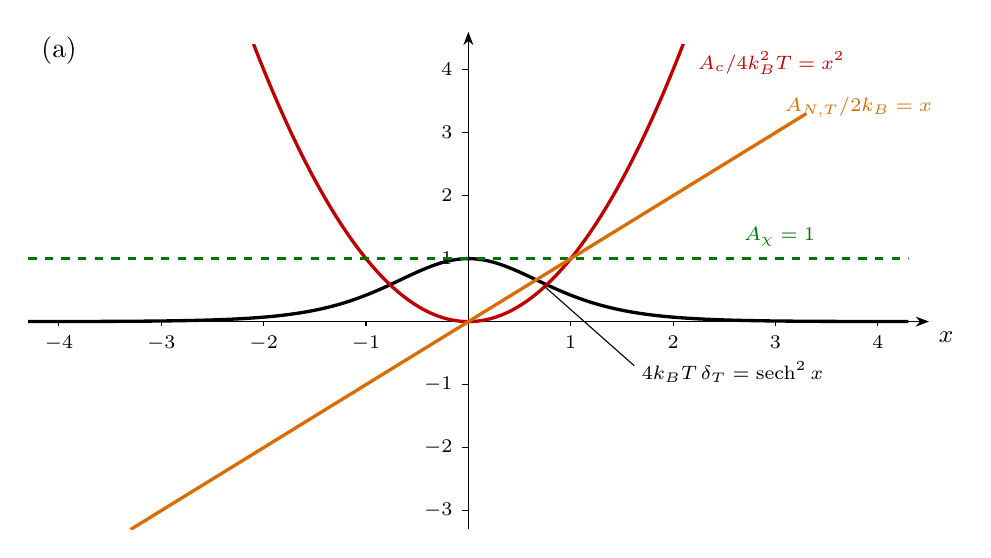
\begin{tikzpicture}[>=Stealth,font=\small,x=1.30cm,y=0.80cm]
  % panel (a): the common window and the observable-specific amplitudes
  \node[font=\normalsize] at (-4.0,4.3) {(a)};
  \draw[->] (-4.3,0) -- (4.5,0) node[below right]{$x$};
  \draw[->] (0,-3.3) -- (0,4.6);
  \foreach \t in {-4,-3,-2,-1,1,2,3,4}
    \draw (\t,0) -- (\t,-0.07) node[below,font=\scriptsize]{$\t$};
  \foreach \t in {-3,-2,-1,1,2,3,4}
    \draw (0,\t) -- (-0.06,\t) node[left,font=\scriptsize]{$\t$};
  \begin{scope}
    \clip (-4.3,-3.3) rectangle (4.3,4.4);
    \draw[very thick,black,domain=-4.3:4.3,samples=180,smooth,variable=\x]
         plot ({\x},{1/(cosh(\x)*cosh(\x))});
    \draw[very thick,red!75!black,domain=-2.1:2.1,samples=120,smooth,variable=\x]
         plot ({\x},{\x*\x});
    \draw[very thick,green!45!black,dashed] (-4.3,1) -- (4.3,1);
    \draw[very thick,orange!85!black,domain=-3.3:3.3,samples=2,variable=\x]
         plot ({\x},{\x});
  \end{scope}
  \node[anchor=west,font=\scriptsize,red!75!black] at (2.15,4.1)
       {$A_c/4k_B^{2}T = x^{2}$};
  \node[anchor=west,font=\scriptsize,orange!85!black] at (3.0,3.4)
       {$A_{N,T}/2k_B = x$};
  \node[anchor=west,font=\scriptsize,green!45!black] at (2.6,1.35)
       {$A_\chi = 1$};
  \node[anchor=west,font=\scriptsize,black] at (1.6,-0.8)
       {$4k_BT\,\delta_T = \operatorname{sech}^{2}x$};
  \draw[black,thin] (1.62,-0.7) -- (0.75,0.55);
\end{tikzpicture}

\vspace{4mm}

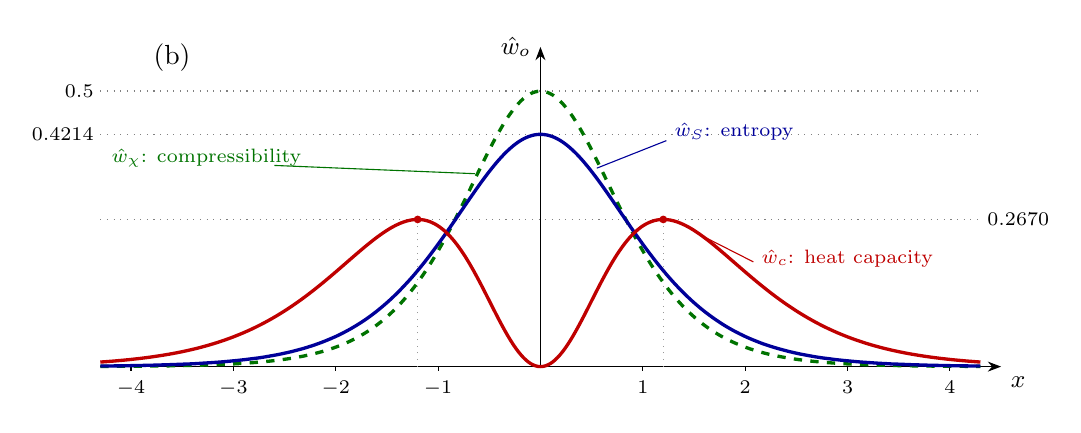
\begin{tikzpicture}[>=Stealth,font=\small,x=1.30cm,y=7.00cm]
  % panel (b): the normalised weights, unit area in x
  \node[font=\normalsize] at (-3.6,0.56) {(b)};
  \draw[->] (-4.3,0) -- (4.5,0) node[below right]{$x$};
  \draw[->] (0,0) -- (0,0.58) node[left]{$\hat w_o$};
  \foreach \t in {-4,-3,-2,-1,1,2,3,4}
    \draw (\t,0) -- (\t,-0.008) node[below,font=\scriptsize]{$\t$};
  \draw[dotted,gray] (-4.3,0.5) -- (4.3,0.5);
  \node[anchor=east,font=\scriptsize,inner sep=1.5pt] at (-4.32,0.5) {$0.5$};
  \draw[dotted,gray] (-4.3,0.4214) -- (4.3,0.4214);
  \node[anchor=east,font=\scriptsize,inner sep=1.5pt] at (-4.32,0.4214) {$0.4214$};
  \draw[dotted,gray] (-4.3,0.2670) -- (4.3,0.2670);
  \node[anchor=west,font=\scriptsize,inner sep=1.5pt] at (4.32,0.2670) {$0.2670$};
  \draw[very thick,green!45!black,dashed,domain=-4.3:4.3,samples=180,smooth,variable=\x]
       plot ({\x},{0.5/(cosh(\x)*cosh(\x))});
  \draw[very thick,blue!60!black,domain=-4.3:4.3,samples=180,smooth,variable=\x]
       plot ({\x},{0.607927*(ln(2*cosh(\x))-\x*tanh(\x))});
  \draw[very thick,red!75!black,domain=-4.3:4.3,samples=180,smooth,variable=\x]
       plot ({\x},{0.607927*\x*\x/(cosh(\x)*cosh(\x))});
  \draw[dotted,gray!80] (1.1997,0) -- (1.1997,0.2670);
  \draw[dotted,gray!80] (-1.1997,0) -- (-1.1997,0.2670);
  \fill[red!75!black] (1.1997,0.2670) circle (1.4pt);
  \fill[red!75!black] (-1.1997,0.2670) circle (1.4pt);
  \node[anchor=south west,font=\scriptsize,blue!60!black,inner sep=2pt]
       at (1.25,0.40) {$\hat w_S$: entropy};
  \draw[blue!60!black,thin] (1.23,0.41) -- (0.55,0.36);
  \node[anchor=south west,font=\scriptsize,red!75!black,inner sep=2pt]
       at (2.10,0.17) {$\hat w_c$: heat capacity};
  \draw[red!75!black,thin] (2.08,0.19) -- (1.55,0.24);
  \node[anchor=south west,font=\scriptsize,green!45!black,inner sep=2pt]
       at (-4.25,0.35) {$\hat w_\chi$: compressibility};
  \draw[green!45!black,thin] (-2.6,0.365) -- (-0.64,0.35);
\end{tikzpicture}

\vspace{4mm}

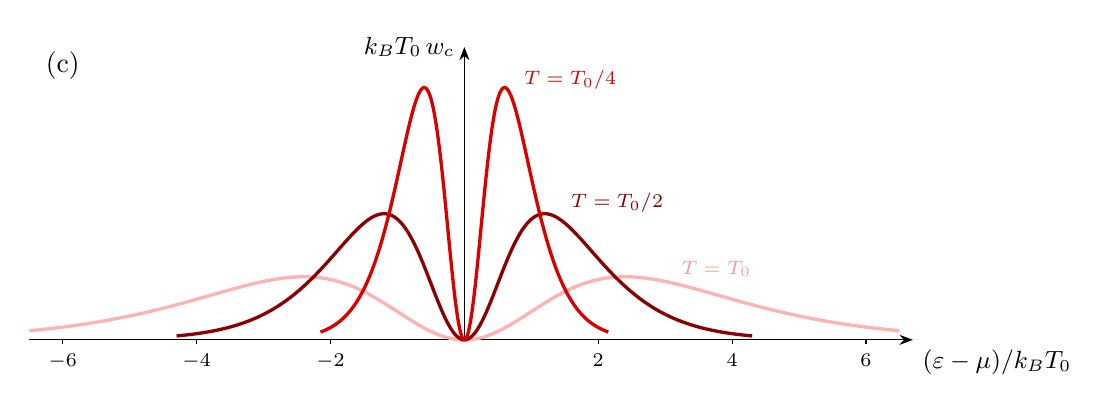
\begin{tikzpicture}[>=Stealth,font=\small,x=0.85cm,y=6.00cm]
  % panel (c): the delta limit of w_c as T -> 0
  \node[font=\normalsize] at (-6.0,0.58) {(c)};
  \draw[->] (-6.5,0) -- (6.7,0) node[below right]{$(\varepsilon-\mu)/k_BT_0$};
  \draw[->] (0,0) -- (0,0.62) node[left]{$k_BT_0\,w_c$};
  \foreach \t in {-6,-4,-2,2,4,6}
    \draw (\t,0) -- (\t,-0.009) node[below,font=\scriptsize]{$\t$};
  \draw[very thick,red!30,domain=-6.5:6.5,samples=200,smooth,variable=\e]
       plot ({\e},{0.303964*(\e/2)^2/(cosh(\e/2)^2)});
  \draw[very thick,red!55!black,domain=-4.3:4.3,samples=200,smooth,variable=\e]
       plot ({\e},{0.607927*(\e)^2/(cosh(\e)^2)});
  \draw[very thick,red!85!black,domain=-2.15:2.15,samples=200,smooth,variable=\e]
       plot ({\e},{1.215854*(2*\e)^2/(cosh(2*\e)^2)});
  \node[anchor=west,font=\scriptsize,red!85!black] at (0.75,0.55) {$T = T_0/4$};
  \node[anchor=west,font=\scriptsize,red!55!black] at (1.45,0.29) {$T = T_0/2$};
  \node[anchor=west,font=\scriptsize,red!40] at (3.1,0.15) {$T = T_0$};
\end{tikzpicture}
\caption{The filter of Eq.~\eqref{eq:filt_integrals} taken apart, against the
symmetric variable $x=(\varepsilon-\mu)/2k_BT$.
(a)~The two factors. The fluctuation window
$ \delta_T = \operatorname{sech}^{2}x/4k_BT = -\partial f/\partial\varepsilon $
(black) is common to every observable: even, non-negative, single-peaked at $\mu$,
of unit area and of width set by $T$ alone. The amplitudes,
Eq.~\eqref{eq:filt_amplitudes}, are shown in dimensionless form: $ A_\chi $ is
constant (a unit change of an occupation moves one particle), $ A_c \propto x^{2} $
(the energy it moves, squared), and $ A_{N,T} \propto x $ is odd, so that
$ (\partial N/\partial T)_\mu $ has no normalised weight of its own.
(b)~The normalised weights of Eq.~\eqref{eq:filt_kernels}, $ \hat w_o = 2k_BT\,w_o $,
each of unit area. The entropy weight peaks at $\mu$ ($ \sigma(0) = \ln2 $: an
orbital with $ n = \tfrac12 $ carries one bit). The heat-capacity weight \emph{vanishes} at
$\mu$, where the amplitude does, and peaks at $|\varepsilon-\mu|=2.3994\,k_BT$.
(c)~The delta limit: $ w_c $ at $ T_0 $, $ T_0/2 $ and $ T_0/4 $, on a fixed energy
axis. The area stays one while the width shrinks $ \propto T $, so
$ w_c \to \delta(\varepsilon - \mu) $; $ w_\chi $ and $ w_S $ do the same.}
\label{fig:filt_kernels}
\end{figure}

\subsection{Why the heat capacity is blind to the levels at \texorpdfstring{$\mu$}{mu}}
\label{sec:filt_blind}

The vanishing of $w_c$ at $\varepsilon=\mu$ --- visible in
Fig.~\ref{fig:filt_kernels}, and easy to miss because it contradicts the usual
picture of $c_V$ as a count of thermally ``available'' states --- is a statement
about \emph{energy fluctuations}. By Eq.~\eqref{eq:filt_C_fluct}, $ k_BT^{2}c_\mu $ is
the variance of $ E - \mu N $ per unit volume, and for independent orbitals it is a
sum of one-orbital energy variances,
\begin{equation}\label{eq:filt_product}
\Var\big[(\varepsilon_\lambda-\mu)\,\hat n_\lambda\big]
\;=\;
\underbrace{(\varepsilon_\lambda-\mu)^{2}}_{\text{energy carried}^{2}}
\;\times\;
\underbrace{n_\lambda(1-n_\lambda)}_{\text{occupancy variance}}\,.
\end{equation}
An orbital contributes to the energy variance only if its occupation fluctuates
\emph{and} each fluctuation moves energy. A level far below $ \mu $ is full with
certainty and a level far above is empty with certainty; neither fluctuates, so
neither contributes, however much energy it would carry. A level exactly at $ \mu $
fluctuates maximally, but a change of its occupation costs zero energy relative
to the reservoir: it moves particles, and so contributes fully to $ \chi_c $, but it
moves no energy, and so contributes nothing to the energy variance or to $ c_\mu $.

The blindness is the additive form of an exact statement. By
Eq.~\eqref{M-eq:filt_mb_response}, $ \chi_c $ and $ c_\mu $ are the variances of two
different conserved quantities, $ \hat N $ and $ \hat{\mathcal{H}} $, over the same distribution
$ p_a $ of eigenstates. Equilibrium mixing among eigenstates that differ in $ N $ but
have the same $ \enrg_a $ --- a particle added or removed at no cost relative to the
reservoir --- contributes to $ \Var(\hat N) $ and nothing to $ \Var(\hat{\mathcal{H}}) $. For independent
fermions those are precisely the fluctuations of the levels at $ \mu $.

\begin{quote}
The heat capacity measures the energy variance of the levels in the fluctuation
window; it sees only the levels whose occupation simultaneously \emph{fluctuates}
and which are \emph{displaced} from $ \mu $, and $|\varepsilon-\mu|=2.4\,k_BT$ is where the
product of the two is largest.
\end{quote}

Availability alone is therefore not sufficient. Each observable asks a different
question of the same window: $ s $ asks how much information is missing about
the occupations of the fluctuating levels, $ \chi_c $ how many particles their fluctuations move, and $ c_\mu $ how
much energy. The same structure explains the exponential decay on both sides,
which is that of the window, $ e^{-|\varepsilon-\mu|/k_BT} $: a level a few $ k_BT $
from $ \mu $ is frozen, and the polynomial prefactors ($ x^{2} $ for $ w_c $, $ 2|x| $
for $ w_S $) only decide how the weights approach that common fate.

\paragraph{The microscopic view of a phase transition.} The variance form says at
once what a divergent response requires. For independent orbitals with a fixed
spectrum each term of Eq.~\eqref{eq:filt_product} is bounded, by
$ (k_BT)^{2}\times0.4392 $ for fermions (Eq.~\eqref{eq:filt_peak}), so
$ \Var(E - \mu N) $ grows at most like the \emph{number} of orbitals: independent
fluctuations add like the steps of a random walk, and the response per unit volume
stays finite (Eq.~\eqref{eq:filt_bound} below). The same holds for $ \Var(N) $ and
$ \Var(M) $. The decomposition
$\Var(\hat{\mathcal H})=\sum_i\Var(\hat h_i)+\sum_{i\neq j}\Cov(\hat h_i,\hat h_j)$
of the variance of a sum of local terms $\hat{\mathcal H}=\sum_i\hat h_i$
shows what is missing: a divergence requires covariances between
the fluctuations of macroscopically many degrees of freedom, and the additive
spectrum, in which the occupations of different orbitals are independent, has none.
In a self-consistent quasiparticle description, where the orbitals remain formally
independent, the same physics appears instead as a spectrum
$ \{\varepsilon_\lambda\} $ that itself moves with $ T $ (Section~\ref{sec:filt_shape}).

\subsection{A power-law density of states}
\label{sec:filt_power}
The value of the filter form is that scale covariance
turns a scale-free spectrum into an exponent by inspection. Let
\begin{equation}\label{eq:filt_powerlaw}
\varrho(\varepsilon)=A\,|\varepsilon-\mu|^{r},\qquad r>-1,
\end{equation}
over a window wide compared with $k_BT$; $r=0$ is a flat band, $r=1$ a Dirac
point in two dimensions, $r=2$ in three, $-1<r<0$ a divergent van Hove-like
enhancement. Substituting into Eq.~\eqref{eq:filt_integrals} with
$\varepsilon-\mu=2k_BTx$ and $d\varepsilon=2k_BT\,dx$, the temperature comes out
of the integral entirely:
\begin{equation}\label{eq:filt_power_C}
c_\mu=k_B A\,(2k_BT)^{r+1}\int_{-\infty}^{\infty}|x|^{r}
x^{2}\operatorname{sech}^{2}x\,dx
\;=\;2k_B A\,(k_BT)^{r+1}\,\Gamma(r+3)\,\eta(r+2),
\end{equation}
where the moment integral is evaluated by expanding
$\operatorname{sech}^{2}x=4\sum_{n\ge1}(-1)^{n-1}n\,e^{-2nx}$ term by term for
$x>0$, giving $\int_0^\infty x^{s-1}\operatorname{sech}^2x\,dx=
4\,\Gamma(s)\,\eta(s-1)/2^{s}$ with $\eta(s)=(1-2^{1-s})\zeta(s)$ the Dirichlet
eta function. At $r=0$ this returns
$2k_BA\,k_BT\,\Gamma(3)\eta(2)=\tfrac{\pi^2}{3}k_B^{2}AT$, i.e.\
Eq.~\eqref{eq:filt_sommerfeld}. So
\begin{equation}\label{eq:filt_exponent}
\;\varrho\sim|\varepsilon-\mu|^{r}\;\Longrightarrow\;c_\mu\sim T^{\,r+1},
\qquad \frac{c_\mu}{T}\sim T^{\,r}\
\end{equation}
The same scale covariance gives an exact equation of state when the power
law holds over the whole band, $\varrho=A\varepsilon^{r}$ from the band
bottom $\varepsilon=0$: integrating Eq.~\eqref{eq:filt_Omega} by parts, as
in the second form of Eq.~\eqref{M-eq:filt_laplace}, with
$\int\varrho=A\varepsilon^{r+1}/(r+1)$ and
$\partial\varphi(u)/\partial\varepsilon=\beta n(u)$,
\[
  \Omega=-\frac{E}{r+1} ,\qquad\text{i.e.}\qquad pV=\frac{E}{r+1} ,
\]
for either statistics and at every $T$ and $\mu$: $pV=\tfrac23E$ for the
non-relativistic gas ($r=\tfrac12$) and $pV=\tfrac13E$ for
photons ($r=2$)~\cite[Sec.~6.2.3]{Honerkamp}.
The entropy carries the \emph{same} exponent with a different amplitude, and the
ratio is exact. Integrating $\int_0^\infty x^{r}\sigma\,dx$ by parts with
Eq.~\eqref{eq:filt_sprime} gives
$\int_0^\infty x^{r}\sigma\,dx=(r+1)^{-1}\int_0^\infty x^{r+2}
\operatorname{sech}^2x\,dx$, so that
\begin{equation}\label{eq:filt_SC}
\;\frac{s}{c_\mu}=\frac{1}{r+1}\qquad\text{exactly, for }
\varrho\propto|\varepsilon-\mu|^{r}\
\end{equation}
The Sommerfeld coincidence $s=c_\mu$ is the special case $r=0$ and nothing more.
In the language of Eq.~\eqref{eq:filt_norm}, $ \Lambda_S = \Lambda_c $ and
$ s/c_\mu $ is the ratio of the $ r $-th absolute moments of the two normalised
weights; at $ r = 2 $ it is $ M_S/M_c = \tfrac13 $, as the table of
Section~\ref{sec:filt_kernels} requires.
Three readings of Eq.~\eqref{eq:filt_SC} are worth having.

For $r>0$ (a semimetal) $s<c_\mu$: states are scarce at $\mu$, and the few that
the window catches are far enough out to be heavily energy weighted.

For $-1<r<0$ the Sommerfeld ratio $c_\mu/T\sim T^{r}$ \emph{diverges} as
$T\to0$, while $c_\mu$ itself still vanishes. This is worth separating, because
the two are routinely conflated: a diverging $\gamma=c/T$ is a statement about
the enhancement of the density of states at $\mu$, not about a divergent heat
capacity, and it is entirely compatible with the third law.

As $r\to-1^{+}$, $s/c_\mu\to\infty$: the entropy stops vanishing as $T\to0$ and
tends to a residual value fixed by the lower cutoff of the scale-free window.
For $r\le-1$ the integral $\int d\varepsilon\,\varrho$ diverges at $\mu$: there would
be infinitely many thermally active levels at arbitrarily low energy, and both
the third law and the normalisability of $\varrho$ fail. The realisable extreme is
therefore $r\to-1$, i.e.\ a residual entropy, and not a divergent $c$.

\paragraph{Metals, Fermi liquids, bad metals.} The exponent $ r $ is a compact
classification of what $ c(T) $ says about the electronic states at the Fermi
level, and it is worth placing the familiar cases on it.
\begin{center}
\small
\begin{tabular}{llll}
\toprule
System & effective $ \varrho $ near $ \mu $ & $ c_{\rm el}(T) $ & $ s/c $ \\
\midrule
simple metal & $ \varrho(\mu) $, band value & $ \gamma T $ & $ 1 $ \\
Fermi liquid & $ (m^\ast/m)\,\varrho_{\rm band}(\mu) $ & $ \gamma^\ast T $ & $ 1 $ \\
marginal Fermi liquid & $ \propto\ln(\Lambda/|\varepsilon-\mu|) $ & $ \propto T\ln(\Lambda/k_BT) $ & $ \simeq 1 $ \\
non-Fermi liquid & $ |\varepsilon-\mu|^{r} $, $ -1<r<0 $ & $ T^{1+r} $ & $ 1/(1+r) > 1 $ \\
2D Dirac (graphene) & $ |\varepsilon-\mu| $ & $ T^{2} $ & $ \tfrac12 $ \\
3D Dirac/Weyl semimetal & $ (\varepsilon-\mu)^{2} $ & $ T^{3} $ & $ \tfrac13 $ \\
\bottomrule
\end{tabular}
\end{center}
In an ordinary metal $ \varrho $ varies on the scale of the bandwidth, $ r = 0 $ to
excellent accuracy, and the filter returns the Sommerfeld law with the band
density of states. In a Landau Fermi liquid the interactions are absorbed into
quasiparticles which are, at low energy, independent orbitals of exactly the type
assumed here, with a renormalised density of states $ \propto m^\ast $; the filter
then measures $ m^\ast $, and in heavy-fermion compounds $ \gamma $ is enhanced by
factors $ 10^{2} $--$ 10^{3} $. What distinguishes a Fermi liquid from free electrons
is not $ c $ alone but its comparison with other windows: the spin susceptibility
sees the same states with amplitude $ m_0^{2} $ instead of $ k_Bx^{2} $, and the
Wilson ratio, $ 1 $ for independent electrons, becomes $ 1/(1 + F_0^{a}) $ with
$ F_0^{a} $ the Landau parameter, typically of order $ 2 $ in heavy fermions. A
\emph{bad metal} --- one whose resistivity exceeds the Mott--Ioffe--Regel limit, so
that no quasiparticle has a mean free path longer than its wavelength --- has no
well-defined orbitals, and Eq.~\eqref{eq:filt_integrals} does not strictly apply.
It remains useful as a definition: a measured $ c(T) $ defines an effective
thermodynamic density of states by inverting the filter (below), and the
characteristic signatures of strange and bad metals, $ c/T \sim \ln(1/T) $ or
$ c/T \sim T^{r} $ with $ r < 0 $, are then read as $ \varrho $ logarithmically or
power-law enhanced at $ \mu $ on the scale of $ k_BT $ --- i.e.\ as the absence of any
energy scale below which the electronic states settle into a Fermi liquid.

\subsection{What the heat capacity determines}
\label{app:cv}
\label{sec:filt_invert_mb}

The thermal map of Section~\ref{M-sec:filt_dist} sends spectral information
into thermal information. This subsection states what is recovered in the
opposite direction from a measured $C_\mu(T)$.

\paragraph{From the heat capacity to the partition function.} By
Eqs.~\eqref{M-eq:filt_mb} and~\eqref{M-eq:filt_CU},
$S(T)=S(0)+\int_0^TC_\mu\,dT'/T'$ and
$\langle\hat{\mathcal H}\rangle(T)=\enrg_0+\int_0^TC_\mu\,dT'$, with
$S(0)=k_B\ln d_0$ (at fixed size the Boltzmann weights tend to $1/d_0$ on
the ground manifold as $T\to0$). Inserting these in
Eq.~\eqref{M-eq:filt_mb} in the form
$\ln\Xi+\beta\enrg_0=S/k_B-\beta(\langle\hat{\mathcal H}\rangle-\enrg_0)$,
\begin{equation}\label{eq:filt_XifromC}
  \ln\frac{e^{\beta\enrg_0}\,\Xi(\beta)}{d_0}
  =\int_0^{T}\frac{C_\mu(T')}{k_BT'}\,dT'-\frac{1}{k_BT}\int_0^{T}C_\mu(T')\,dT' ,
  \qquad
  \frac{e^{\beta\enrg_0}\,\Xi(\beta)}{d_0}=\Big\langle\frac{\rho(\enrg_0+\,\cdot\,)}{d_0}\,,\,e_\beta\Big\rangle :
\end{equation}
the heat capacity at all temperatures gives the Laplace transform of the
distribution $\cE\mapsto\rho(\enrg_0+\cE)/d_0$ of the excitation energy
$\cE:=\enrg-\enrg_0\ge0$, for all $\beta>0$.

\begin{proposition}[What $C_\mu(T)$ determines]\label{prop:invert}
For any Hamiltonian, the function $C_\mu(T)$, $0<T<\infty$, at fixed $\mu$
determines the distribution $\rho(\enrg_0+\cE)/d_0$, i.e.\ all excitation
energies $\enrg_a-\enrg_0$ of $\hat{\mathcal H}$ and all ratios of degeneracies
$d_n/d_0$. It does not determine $\enrg_0$ and $d_0$.
\end{proposition}
\begin{proof}
A measure on $[0,\infty)$ is determined by its Laplace transform (Lerch's
theorem\footnote{\emph{Lerch's theorem}: if two functions have the same
Laplace transform for all $\beta>\beta_0$ (it suffices: at the equidistant
points $\beta_0+n\eta$, $n=0,1,2,\dots$), they are equal almost everywhere;
in the present form, the transform $\int e^{-\beta\cE}d\cN(\cE)$ determines
the non-decreasing function $\cN$. The idea of the proof: with
$x=e^{-\eta\cE}$ the transforms at the equidistant points are the moments
$\int_0^1x^{n}(\dots)\,dx$ of a function on $[0,1]$, and a continuous
function all of whose moments vanish is zero, since it can be approximated
uniformly by polynomials (Weierstrass)~\cite{Widder}.}), which with
Eq.~\eqref{eq:filt_XifromC} gives the first statement. For the second,
$C_\mu=\Var(\hat{\mathcal H})/k_BT^{2}$ is unchanged by a shift of all
levels, $\enrg_a\to\enrg_a+{\rm const}$, and by a multiplication of all
degeneracies by a common factor, $\rho\to{\rm const}\times \rho$.
\end{proof}
What is determined is the distribution, i.e.\ the measure $d\cN$, not values
of $\rho$ at points, which do not exist. The two undetermined constants are
fixed by other data: $d_0$ by the entropy sum rule
$\ln(D/d_0)=\int_0^\infty C_\mu\,dT/k_BT$, Eq.~\eqref{eq:filt_sumrule}, if the
dimension $D$ of the Fock space is known; and $\enrg_0$, as a function of
$\mu$, by the equation of state, $\langle\hat N\rangle=-\partial\Omega/\partial\mu$.

\paragraph{What needs other observables.} The heat capacity contains no
information on the dependence of the spectrum on a field. By
Eqs.~\eqref{M-eq:filt_param} and~\eqref{M-eq:filt_gA},
$\Xi\,\langle\hat A\rangle=\langle \rho_A,e_\beta\rangle$, so the conjugate
quantity $\langle\hat A\rangle(T)$, together with $\Xi$, determines by the
same theorem the weighted density of states
$\rho_A=\sum_aA_{aa}\,\delta(\enrg-\enrg_a)$, i.e.\ the slopes of the levels in the
field; the susceptibility $\chi_{AA}(T)$ likewise determines
$\partial^{2}\rho/\partial \hfield^{2}$. The eigenvectors enter the thermodynamics
only through these derivatives of the levels.

\paragraph{The inverse map is not continuous.} The inversion is exact but
severely ill-posed: the test function $e_\beta$ varies on the scale $k_BT$,
so two spectra that differ only in structure narrower than $k_BT_{\min}$,
with $T_{\min}$ the lowest temperature measured, have heat capacities that
differ by an arbitrarily small amount. Such structure is beyond the reach of
thermodynamics and needs a spectroscopy. What is recovered robustly is the
low-temperature asymptotic form, Eq.~\eqref{M-eq:filt_sinv}, each term of
which fixes one term in the low-energy expansion of $\ln\cN$. The additive
case, in which $c(T)$ can be inverted for the single-particle density of
states, is treated in Section~\ref{sec:filt_invert}.

\subsection{Inverting the filter}
\label{sec:filt_invert}

The exact inversion of $ c(T) $ for the many-body density of states was given in
Section~\ref{sec:filt_invert_mb}; what follows is the additive case.
Since a measured $ c(T) $ is then a linear integral transform of
$ \varrho $, it is natural to ask whether the transform can be inverted to recover $ \varrho $,
especially at low energy, where the window is narrow. The answer has three parts.

\emph{What can be recovered.} The weight $ w_c $ is even, so $ c_\mu $ determines
only the symmetrised density of states $ \varrho_s(\omega) =
\tfrac12[\varrho(\mu + \omega) + \varrho(\mu - \omega)] $, $ \omega > 0 $; the
antisymmetric part is invisible to it and must be obtained from an odd response, such
as $ (\partial N/\partial T)_\mu $ of Eq.~\eqref{eq:filt_amplitudes} or, in practice, the
thermopower. Combining several even weights cannot recover the antisymmetric part,
since they all see the same $ \varrho_s $; but, as shown at the end of this
subsection, it does help to determine $ \varrho_s $ itself.

\emph{Exact inversion.} Write $ \tau = 2k_BT $ and $ k(y) = y^{2}\operatorname{sech}^{2}y $,
so that, folding the integral over $ \varepsilon $ onto $ \omega = |\varepsilon - \mu| $,
\[
  c_\mu(\tau) = 2k_B\int_0^{\infty} d\omega\;\varrho_s(\omega)\,k(\omega/\tau) .
\]
Scale covariance makes this a convolution on a \emph{logarithmic} energy axis, which
the Mellin transform diagonalises. Multiplying by $ \tau^{-s-1} $, integrating over
$ \tau $ and substituting $ y = \omega/\tau $ in the inner integral,
\[
  \int_0^{\infty} d\tau\;\tau^{-s-1}c_\mu(\tau)
  = 2k_B\,G(s)\int_0^{\infty} d\omega\;\omega^{-s}\varrho_s(\omega),
\]
with
\[
  G(s) = \int_0^{\infty} dy\; y^{s-1}k(y) = \frac{4\,\Gamma(s+2)\,\eta(s+1)}{2^{s+2}} ,
\]
the last by the series used in Eq.~\eqref{eq:filt_power_C}. The Mellin transform of
$ \varrho_s $ is thus the Mellin transform of the data divided by the known function
$ G(s) $, and an inverse Mellin transform returns $ \varrho_s(\omega) $. In principle,
then, $ c(T) $ over all temperatures determines $ \varrho_s $ uniquely.

\emph{Why it is ill-posed in practice.} Along the line $ s = \sigma + it $, the
factor $ \Gamma(s+2) $ in $ G $ decays as $ e^{-\pi|t|/2} $. Dividing by $ G $ therefore
amplifies the components of the data that oscillate rapidly in $ \ln T $
exponentially in their frequency, and any noise there swamps the reconstruction.
The resolution is fixed on a logarithmic scale: at temperature $ T $ the weight
samples $ \varrho $ around $ |\omega| \approx 2.4\,k_BT $ with a width of the same order, so
structure at energy $ \omega $ can be resolved only to within a factor of order one
in $ \omega $ itself. Lowering $ T $ improves the \emph{absolute} resolution, since the
window shrinks, but not the \emph{relative} one. What survives robustly is the
low-temperature asymptotic series. Matching Eq.~\eqref{eq:filt_power_C} term by term,
\[
  c_\mu(T) \simeq \sum_r a_r T^{r+1}
  \quad\Longleftrightarrow\quad
  \varrho_s(\omega) \simeq \sum_r A_r\,\omega^{r},
  \qquad
  A_r = \frac{a_r}{2k_B^{r+2}\,\Gamma(r+3)\,\eta(r+2)} ,
\]
so the leading power and amplitude of $ c(T) $ fix the leading behaviour of $ \varrho_s $
at low energy exactly, and each further term the next correction. Fine structure
in $ \varrho $ narrower than a few $ k_BT $ at the lowest measured temperature is beyond the
reach of thermodynamics and requires a spectroscopy (tunnelling, photoemission)
whose resolution is not tied to $ T $.

\emph{Combining observables at low temperature.} A single observable measured at a
single temperature returns one number, and Eq.~\eqref{eq:filt_delta_limit} shows
which combination of the Taylor coefficients of $ \varrho $ at $ \mu $ it is. Different
observables return \emph{different} combinations, because their weights have
different moments, and a set of observables measured at the same temperature can
therefore be solved for the coefficients individually. Write
$ \varrho_k := \varrho^{(k)}(\mu) $ for the $ k $-th derivative and divide each observable
by its flat-band prefactor, $ \hat o := o/\Lambda_o $. Taylor-expanding $ \varrho $ about
$ \mu $ under the integral of Eq.~\eqref{eq:filt_norm}, and using that the even weights
have vanishing odd moments,
\[
  \hat o(T) = \sum_{k\geq0}\frac{\varrho_{2k}}{(2k)!}\,(2k_BT)^{2k}\,m^{(2k)}_o ,
  \qquad
  m^{(2k)}_o := \int dx\; x^{2k}\,\hat w_o(x) ,
\]
an exact linear system in the unknowns $ \varrho_0, \varrho_2, \varrho_4, \dots $, with
coefficients $ m^{(2k)}_o $ known once and for all. To the first non-trivial order the
second moments of the table above give, for the three normalised observables
\[
  \hat\chi := \chi_c = \frac{\chi_s}{m_0^{2}} , \qquad
  \hat c := \frac{c_\mu}{\pi^{2}k_B^{2}T/3} , \qquad
  \hat s := \frac{s}{\pi^{2}k_B^{2}T/3} ,
\]
the system
\[
  \begin{pmatrix} \hat\chi \\ \hat c \\ \hat s \end{pmatrix}
  = \begin{pmatrix} 1 & \pi^{2}/6 \\ 1 & 7\pi^{2}/10 \\ 1 & 7\pi^{2}/30 \end{pmatrix}
  \begin{pmatrix} \varrho(\mu) \\ (k_BT)^{2}\varrho''(\mu) \end{pmatrix}
  + O(T^{4}) .
\]
Any two rows determine both unknowns. From the compressibility and the heat
capacity,
\[
  \varrho(\mu) \simeq \frac{21\,\hat\chi - 5\,\hat c}{16} ,
  \qquad
  \varrho''(\mu) \simeq \frac{15}{8\pi^{2}}\,\frac{\hat c - \hat\chi}{(k_BT)^{2}} ,
\]
so that the curvature of the density of states at the Fermi level is read off from
the \emph{difference} between the normalised heat capacity and the normalised
compressibility (or spin susceptibility) at one temperature, without fitting a
temperature dependence; for independent electrons the Wilson ratio
$ R_W = \hat\chi/\hat c $ deviates from $ 1 $ by $ -(8\pi^{2}/15)(k_BT)^{2}\varrho''/\varrho $.
The third row is then a consistency check: the residual
$ \hat s - \tfrac18(7\hat\chi + \hat c) $, which vanishes to this order, measures the
$ O(T^{4}) $ terms.
The antisymmetric part follows from the odd observable: with
$ A_{N,T} = (\varepsilon - \mu)/T $ and the second moment of the window,
\[
  \frac{1}{V}\left(\frac{\partial N}{\partial T}\right)_{\mu}
  = \frac{\pi^{2}}{3}k_B^{2}T\,\varrho'(\mu) + O(T^{3}) ,
\]
which fixes $ \varrho'(\mu) $. With $ J $ even observables and the expansion truncated
after $ J $ even coefficients, the system is square, and it is solvable whenever the matrix
of moments is non-singular; including several temperatures enlarges the system and
over-determines it.

Two limitations should be kept in view. First, the moment matrix is ill-conditioned:
the weights are all of similar shape, their moments differ by factors of order one,
and the information about $ \varrho_2 $ enters at relative order
$ (k_BT)^{2}\varrho''/\varrho $, so the differences of observables must be measured to that
relative accuracy; each further coefficient costs another factor $ (k_BT)^{2} $. This
is the same ill-posedness as that of the Mellin inversion, now in a finite-dimensional
form. Second, the combination presupposes that all observables see the same
independent levels. In an interacting system they need not: in a Fermi liquid
$ \chi_s $ and $ c_\mu $ are renormalised differently, the Wilson ratio departs from $ 1 $
already at $ T = 0 $ (Section~\ref{sec:filt_power}), and the difference $ \hat c - \hat\chi $
then measures the Landau parameter $ F_0^{a} $ rather than $ \varrho''(\mu) $. The
procedure is exact for quadratic Hamiltonians and should be read, otherwise, as a
definition of effective densities of states, one per observable, whose differences
are themselves informative.

\subsection{Reading the shape of \texorpdfstring{$c(T)$}{c(T)}}
\label{sec:filt_shape}

The elementary reading of the specific heat is calorimetric: $c=\dbar Q/dT$, so
$\Delta T\simeq\Delta Q/c$, and a large $c$ means that a given amount of heat
raises the temperature little because the system has somewhere to put it. The
filter form makes this quantitative and corrects it in one respect: ``somewhere
to put it'' is neither the total number of states nor the number below $k_BT$,
but the number that $w_c$ actually weighs. With that correction, the standard
readings of the \emph{shape} of $c(T)$ follow, and they are worth listing because
the practical use of a measured $c(T)$ consists in running them backwards.

\paragraph{Rise.} An increase of $c$ with temperature means that the weight is
dilating into a region of higher level density, so that each further unit of
temperature activates more excitations than the last. Equation~\eqref{eq:filt_exponent}
is the quantitative version: a pure power $c\sim T^{r+1}$ is the case in which the
spectrum presents no scale for the dilation to encounter, and the measured
exponent returns $r$ directly.

\paragraph{Plateau.} A temperature-independent $c$ is the marginal case
$r+1=0$ of Eq.~\eqref{eq:filt_exponent}, i.e.\ $\varrho\propto|\varepsilon-\mu|^{-1}$,
for which the power-law integrals fail logarithmically and the level count in a
window of width $\Delta$ grows as $\ln\Delta$ rather than as a power. Since
Section~\ref{sec:filt_power} showed $r\le-1$ to be non-normalisable, a plateau
cannot extend to $T\to0$: it is necessarily the behaviour \emph{between} the two
cutoffs of a scale-free window, which is what a geometric hierarchy of levels
produces, and it terminates at the bottom in the residual entropy that the lower
cutoff fixes. A plateau is thus considerably more informative than it looks --- it
identifies logarithmic counting, and it comes with a prediction for where it must
end.

\paragraph{Peaks, and the staircase caveat.} A peak is the generic shape whenever
the spectrum has a largest relevant scale. Its rising side is the filling of the
window; its falling side is \emph{exhaustion} --- once $k_BT$ exceeds the largest
splitting in the group of levels concerned, they are all equally populated, their
occupations stop changing with temperature, and by
Eq.~\eqref{eq:filt_product} the sector ceases to absorb heat. The bookkeeping is
the entropy sum rule, which follows immediately from $c=T(\partial s/\partial T)$ and
holds for any Hamiltonian:
\begin{equation}\label{eq:filt_sumrule}
\int_0^{\infty}c(T)\,\frac{dT}{T}=s(\infty)-s(0).
\end{equation}
The area under $c/T$ \emph{counts the states released}, and a peak is the only
way a finite count can be released over a finite range.

The caveat concerns the frequent claim that a tiered spectrum gives a staircase
in $c$. It does not. A set of \emph{well-separated} tiers gives a staircase in
$s(T)$, whose step heights are the logarithms of the tier multiplicities, and a
\emph{sequence of peaks} in $c(T)$, one per tier, with $c$ returning towards zero
between them. A staircase in $c$ requires the tiers to overlap on a logarithmic
temperature axis, i.e.\ to be dense enough to produce the logarithmic counting of
the previous paragraph.

\paragraph{High temperature.} Whether $c$ must vanish as $T\to\infty$ is settled
by the same sum rule, and the answer is conditional. If the spectrum is bounded
and the degrees of freedom have finite dimension, then $s(\infty)$ is bounded by
$k_B\ln(\dim\mathcal{H})/V$ and Eq.~\eqref{eq:filt_sumrule} forces $c\to0$. The
explicit form, for any Hamiltonian with a finite Fock space, is the tail
$c_\mu=\Var_\infty(\hat{\mathcal H})/Vk_BT^{2}+O(T^{-3})$, with $\Var_\infty$
the variance of the spectrum over all states with equal weights; in the
additive case it is the Schottky tail obtained from
Eq.~\eqref{eq:filt_C} at $x_\lambda\to0$,
\begin{equation}\label{eq:filt_schottky}
c_\mu\;\xrightarrow[T\to\infty]{}\;\frac{k_B}{V}\sum_\lambda x_\lambda^{2}
=\frac{\Var_\infty(E-\mu N)}{Vk_BT^{2}}\;\propto\;\frac{1}{T^{2}},
\end{equation}
with a finite coefficient. Degrees of freedom of unbounded spectrum and unbounded
occupation --- harmonic modes --- instead settle at the equipartition value $k_B$
per mode, with $S$ growing as $\ln T$ without bound. That value is not an
exception to the framework but a reading of it: the per-orbital Bose heat capacity of
Section~\ref{sec:filt_twolevel} is $k_Bu^{2}n(1+n)$, and since $n\simeq1/u$ as
$u\to0$ it tends to $k_B$ rather than vanishing there, which is equipartition. A vanishing
high-temperature $c$ is thus a statement about the finite dimension of the local
Hilbert space, not a thermodynamic requirement.

\paragraph{Divergence.} This is the informative case, and the filter form settles
what it can and cannot mean. Since Eq.~\eqref{eq:filt_C} is a sum of terms each
bounded by Eq.~\eqref{eq:filt_peak}, the bound holds term by term:
\begin{equation}\label{eq:filt_bound}
\;c_\mu\;\leq\;0.4393\,k_B\times(\text{number of orbitals per unit volume})\
\end{equation}
at \emph{every} temperature. The constant is the fermionic one; the same argument
bounds the per-orbital Bose heat capacity by its $u\to0$ value $k_B$ and the Boltzmann one by
$4e^{-2}k_B=0.5413\,k_B$, so in every case the bound is $\mathcal{O}(k_B)$ per
mode. A lattice model with finitely many modes per site and a
temperature-independent spectrum therefore has an $\mathcal{O}(k_B)$ heat
capacity per site and cannot diverge at all. (Without additivity the bound is
replaced by the decomposition of $ \Var(\hat{\mathcal{H}}) $ into the
variances and covariances of the local terms of $ \hat{\mathcal{H}} $:
$ \Var(\hat{\mathcal{H}})/V $ stays finite unless the covariances become
long-ranged.) Every divergence is consequently a
statement that the spectrum itself \emph{moves}: with temperature, through
self-consistency --- an order parameter that reconstructs the band as it
re-equilibrates --- or with a control parameter, through the accumulation of
level crossings at a transition. And a divergence as $T\to0$ is excluded on the
second, independent ground of Section~\ref{sec:filt_power}: it would require
$r<-1$, hence a non-normalisable $\varrho$ and a violation of the third law. What
diverges in a non-Fermi-liquid regime is the Sommerfeld ratio $c/T\sim T^{r}$,
not $c$.

\begin{remark}
Equation~\eqref{eq:filt_bound} is a statement about non-interacting levels, and
the escape clause in it --- ``temperature-independent spectrum'' --- is where all
the interesting physics of strongly correlated systems lives. It is nevertheless
the right null hypothesis: any claim of an anomalously large $c$ carries the
burden of identifying either the extra orbitals or the moving spectrum that
produces it.
\end{remark}

\bibliographystyle{plain}
\bibliography{thermo_dos}

\end{document}
